%
% FH Technikum Wien
% !TEX encoding = UTF-8 Unicode
%
% Erstellung von Master- und Bachelorarbeiten an der FH Technikum Wien mit Hilfe von LaTeX und der Klasse TWBOOK
%
% Um ein eigenes Dokument zu erstellen, müssen Sie folgendes ergänzen:
% 1) Mit \documentclass[..] einstellen: Master- oder Bachelorarbeit, Studiengang und Sprache
% 2) Mit \newcommand{\FHTWCitationType}.. Zitierstandard festlegen (wird in der Regel vom Studiengang vorgegeben - bitte erfragen)
% 3) Deckblatt, Kurzfassung, etc. ausfüllen
% 4) und die Arbeit schreiben (die verwendeten Literaturquellen in Literatur.bib eintragen)
%
% Getestet mit TeXstudio mit Zeichenkodierung ISO-8859-1 (=ansinew/latin1) und MikTex unter Windows
% Zu beachten ist, dass die Kodierung der Datei mit der Kodierung des paketes inputenc zusammen passt!
% Die Kodierung der Datei twbook.cls MUSS ANSI betragen!
% Bei der Verwendung von UTF8 muss dnicht nur die Kodierung des Dokuments auf UTF8 gestellt sein, sondern auch die des BibTex-Files!

\documentclass[MGS,Master,english]{twbook}%\documentclass[Bachelor,BMR,german]{twbook}
\usepackage[utf8]{inputenc}
\usepackage[T1]{fontenc}
\usepackage{cite}
\usepackage[numbers]{natbib}
\usepackage{booktabs}
\usepackage{wrapfig}
\usepackage{graphicx}

%
% Bitte in der folgenden Zeile den Zitierstandard festlegen
\newcommand{\FHTWCitationType}{IEEE} % IEEE oder HARVARD möglich - wenn Sie zwischen IEEE und HARVARD wechseln, bitte die temorären Dateien (aux, bbl, ...) löschen
%
\ifthenelse{\equal{\FHTWCitationType}{HARVARD}}{\usepackage{harvard}}{\usepackage{bibgerm}}

% Definition Code-Listings Formatierung:
\usepackage[final]{listings}
\lstset{captionpos=b, numberbychapter=false,caption=\lstname,frame=single, numbers=left, stepnumber=1, numbersep=2pt, xleftmargin=15pt, framexleftmargin=15pt, numberstyle=\tiny, tabsize=3, columns=fixed, basicstyle={\fontfamily{pcr}\selectfont\footnotesize}, keywordstyle=\bfseries, commentstyle={\color[gray]{0.33}\itshape}, stringstyle=\color[gray]{0.25}, breaklines, breakatwhitespace, breakautoindent}
\lstloadlanguages{[ANSI]C, C++, [gnu]make, gnuplot, Matlab}

%Formatieren des Quellcodeverzeichnisses
\makeatletter
% Setzen der Bezeichnungen für das Quellcodeverzeichnis/Abkürzungsverzeichnis in Abhängigkeit von der eingestellten Sprache
\providecommand\listacroname{}
\@ifclasswith{twbook}{english}
{%
    \renewcommand\lstlistingname{Code}
    \renewcommand\lstlistlistingname{List of Code}
    \renewcommand\listacroname{List of Abbreviations}
}{%
    \renewcommand\lstlistingname{Quellcode}
    \renewcommand\lstlistlistingname{Quellcodeverzeichnis}
    \renewcommand\listacroname{Abkürzungsverzeichnis}
}
% Wenn die Option listof=entryprefix gewählt wurde, Definition des Entyprefixes für das Quellcodeverzeichnis. Definition des Macros listoflolentryname analog zu listoflofentryname und listoflotentryname der KOMA-Klasse
\@ifclasswith{scrbook}{listof=entryprefix}
{%
    \newcommand\listoflolentryname\lstlistingname
}{%
}
\makeatother
\newcommand{\listofcode}{\phantomsection\lstlistoflistings}

% Die nachfolgenden Pakete stellen sonst nicht benötigte Features zur Verfügung
\usepackage{blindtext}

%
% Einträge für Deckblatt, Kurzfassung, etc.
%
\title{%
	Using LLVM/Clang to to abide cache conscious data layout principles, yet maintain the abstraction level of Object Oriented Programming\\
	\large How compiler technology could possibly build a bridge between conflicting programming paradigms}
\author{Julian Müller, BSc.}
\studentnumber{1610585015}
%\author{Titel Vorname Name, Titel\and{}Titel Vorname Name, Titel}
%\studentnumber{XXXXXXXXXXXXXXX\and{}XXXXXXXXXXXXXXX}
\supervisor[Supervisor]{Stefan Reinalter, DI}
\secondsupervisor[Second Supervisor]{Prof. Alexander Hofmann, DI}

\place{Wien}

\outline{This work will prospect the possibility of using compiler technology as a mediator between the conflicting programming paradigms/philosophies \textit{OOP} and \textit{DoD}.\\While Object oriented programming is often praised for its benefits on abstraction and maintainability, it encourages programmers to design inefficient datalayouts. Specifically in game engineering, where performance is a constitutive factor for a product's success, data oriented solutions and influences are on the rise. While it is debated, wether or not performant data layouts inevitably entail challenging maintenance, surely the base concepts of \textit{objects} are well observable in a game. Therefore this will be an attempt to make object oriented programming a valid option for ever rising demands on performance.\\
To do so this thesis will investigate key concepts of both paradigms, as well as hardware specifics in modern computer architectures to explicate the reasons for their good/bad interaction with the hardware.\\
A prototypical implementation of a source-to-source transformation tool called \textit{COOP} (\textbf{C}ache friendly \textbf{O}bject \textbf{O}riented \textbf{P}rogramming), developed in Clang's LibTooling environment, will determine wether or not compiler technology can be used to achieve a performance optimization on a classically OOP abidant target code base.}
\keywords{Object Oriented Programming, OOP, Structure Of Arrays, SOA, Data Oriented Design, Compiler, LLVM, Clang}

\acknowledgements{TODO dankscheeee}

\begin{document}

%Festlegungen für den HARVARD-Zitierstandard
\ifthenelse{\equal{\FHTWCitationType}{HARVARD}}{
\bibliographystyle{Harvard_FHTW_MR}%Zitierstandard FH Technikum Wien, Studiengang Mechatronik/Robotik, Version 1.2e
\citationstyle{dcu}%Correct citation-style (Harvardand, ";" between citations, "," between author and year)
\citationmode{abbr}%use "et al." with first citation

%Englisch
\newcommand{\citepic}[1]{(Source: \protect\cite{#1})}%Zitat: Bild
\newcommand{\citefig}[2]{(Source: \protect\cite{#1}, p. #2)}%Zitat: Bild aus Dokument

\newcommand{\citefigm}[2]{(Source: taken with modification from \protect\cite{#1}, p. #2)}%Zitat: modifiziertes Bild aus Dokument
\newcommand{\citep}{\citeasnoun}%In-Line Zitiat entweder mit \citep{} oder \citeasnoun{}
\newcommand{\acessedthrough}{Available at:}%Für URL-Angabe
\newcommand{\acessedthroughp}{Available through:}%Für URL-Angabe (Geschützte Datenbank, Zugriff durch FH)
\newcommand{\acessedat}{Accessed}%Für URL-Datum-Angabe
\newcommand{\singlepage}{p.}%Für Seitenangabe (einzelne Seite)
\newcommand{\multiplepages}{pp.}%Für Seitenangabe (mehrere Seiten)
\newcommand{\chapternr}{Ch.}%Für Kapitelangabe
\renewcommand{\harvardand}{\&}%Harvardand in Zitaten
\newcommand{\abstractonly}{Abstract only}
\newcommand{\edition}{~edition}%Edition -> note, that you have to write "edition = {2nd},"!
}

%CUSTOM
\newcommand{\mc}[1]{\cite{#1}}
\newcommand{\mcp}[2]{\cite[p. #2]{#1}}
\newcommand{\mcpic}[1]{(Source: \mc{#1})}
\newcommand{\mcppic}[2]{(Source: \mcp{#1}{#2})}

\newcommand{\reffig}[1]{Fig. \ref{#1}}
\newcommand{\reffigp}[1]{(see \reffig{#1})}

\newcommand{\refcode}[1]{Code \ref{#1}}
\newcommand{\refcodep}[1]{(see \refcode{#1})}

\newcommand{\refsec}[1]{Section \ref{#1}}
\newcommand{\refsecp}[1]{(see \refsec{#1})}

\newcommand{\reftable}[1]{Table \ref{#1}}
\newcommand{\reftablep}[1]{(see \reftable{#1})}


%MATH CUSTOM
\providecommand{\myceil}[1]{\left \lceil #1 \right \rceil }
\providecommand{\myfloor}[1]{\left \lfloor #1 \right \rfloor }

\maketitle

%
% .. und hier beginnt die eigentliche Arbeit. Viel Erfolg beim Verfassen!
%
\chapter{Conflicting Paradigms}
Numerous programming paradigms exist for even more general programming languages. Each of them come with different perks and offer different perspectives for a problem. Different programming paradigms, however do not necessarily exclude each other. Languages like \textit{Scala} for example combine functional and object oriented programming.\\
This thesis will specifically concentrate on \textit{Object-Oriented Programming} (OOP) and \textit{Data-Oriented Design} (DoD). Whether or not data oriented design is even to be considered a programming paradigm is debatable \mcp{fabian}{1}. However its fundamental ideas (specifically concerning data layout) conflict with those of existing paradigms like OOP. Therefore to maintain consistency in this manner of comparison, it will be mentioned accordingly.\\ 
Depending on the domain, certain programmers will have different answers to the question which of both should be preferred. Each party will make compelling arguments to why their choice is mandatory. This is because those paradigms (partially) solve different problems and therefore offer dissenting perspectives on problems and their respective solutions for them.
To understand why \textit{Object Oriented Programming} and \textit{Data Oriented Design} are rather cannibalistic to each other, it is important to first have a look at what they are trying to solve, independently.

\section{Object Oriented Programming / AOS}\label{OOP}
Starting with punch cards, each iteration of new programming generations provided new forms of abstraction for programmers, be it control flow statements, type systems, data structures like native arrays. When machine code started to simplify operations, FORTRAN partly introduced portability as early as 1957; LISP introduced symbolic processing and automated memory management until finally Simula/67 introduced objects in the 1960s \mc{louden}\mc{hopl}.
Object Oriented Programming could not be called popular until the 1970s or 1980s, when Stroustrup created C++. Originally OOP was meant to be the way to go for creating graphics based applications  \mc{about_oop}. This makes sense, since tree like data structures (e.g. GUIs) containing entities with shared behavior can easily be described with polymorphism.\\
OOP shines, whenever the problem to be modeled can be abstracted to one or more base classes, that define shared state and/or behavior. Even though some languages allow for a subclass to "\textit{exclude variables and/or methods which would otherwise have been inherited from the superclass(es)}" \mcp{what_is_oop}{4} the general concept of objects usually includes derivation and extending base behavior.\\
OOP quickly established and rooted itself in the industry without solely being used on graphics applications. This is due to the fact, that it represents a world model, we are taught since elementary school. We are familiar with \textit{is-a} relations ever since we learned that despite dissenting traits, both Labradors and Pugs are dogs. Arguably abstraction is one of - if not - the most important disciplines in programming \mcp{ghezzi}{5}. Since programs oftentimes try to model real life information, OOP delivers an easy to grasp, quick-to-learn approach to do so. That is also the reason, why there are so many OOP programmers around the world. Without trying to evaluate whether or not OOP's way of abstraction is superior to DoD, it is undoubtedly the more prominent one, especially for virtually any other profession than a programmer/computer scientist \reffigp{lang_ratings}.
\begin{figure}[!htbp]
	\centering
	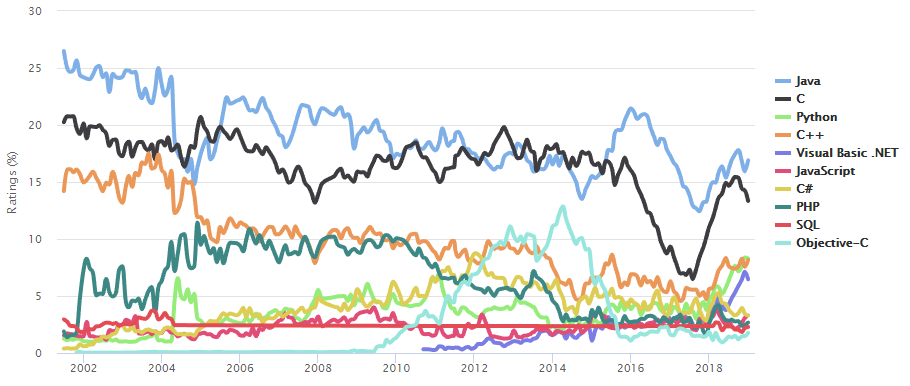
\includegraphics[width=1.0\linewidth]{PICs/lang_ratings}
	\caption{Most popular programming languages throughout the years \mcpic{lang_ratings}.}\label{lang_ratings}
\end{figure}
 This is however where OOP and modern computer architectures do not get along, so to say. OOP offers an elegant way to intuitively model an issue into code, but doing so it encourages us to implement our data in an inefficient way. Inefficient because creating monolithic models of our data usually lack cohesion, which means, that the classes' members tend to not be related/dependent \mc{cohesion} - at least in terms of computational order or domain affiliation. In a home office application, juggling a few dozens of entities every other minute, this will not appear as a problem. And in this case it might be preferable to program such application in a strict object oriented way, since the development can be done fast and reliably even by a novice. On the other hand and especially in the game development industry OOP has proven to result in poorly performing software, due to inefficient data layouts. Because especially for games where oftentimes lots of game entities are being processed several times per second: "\textit{data is performance}" \mcp{nystrom}{272}.\\
 \begin{lstlisting}[language=C++,numbers=none,name={Example of some hierarchical POD class definitions},label={pods}]
struct Obj {				struct Human : Obj {			struct NPC : Human {
	float xyz[3];				char *name;						int mood;
	float vel[3];				int age;						};
};								};

NPC npc_arr[3];
 \end{lstlisting}
The abbreviation \textit{AOS} stands for \textit{Array Of Structures}\mc{intel} and it describes, what usually happens with Object Oriented Programming.\\
Considering the rather arbitrary C++ class definitions in \refcode{pods} the \textit{npc\_arr} will occupy memory according to \reffig{npcs_in_memory} (disregarding any \textit{padding}).
\begin{figure}[!htbp]
	\centering
	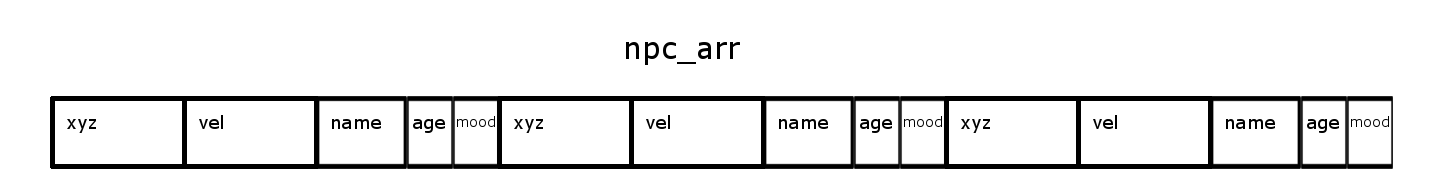
\includegraphics[width=1.0\linewidth]{PICs/npcs_in_memory}
	\caption{Visualization of how \textit{npc\_arr} will exist in memory}\label{npcs_in_memory}
\end{figure}
This is quite literally an array of structures - hence the notation \textit{AOS}. The following sections \ref{cpu_caches} and \ref{dod} will elaborate on \textit{why} exactly this way of thinking/way of abstraction and its respective layout in memory is inefficient.

\section{CPU Caches and why they don't \textit{fit} objects}\label{cpu_caches}
The data layouts typically found when programming with objects and classes, are not inefficient because they lack logic. "\textit{Each human - including NPCs - will have positional traits}", is semantically correct. In fact it seems rather unfortunate, that modern computer architectures ca not deal well with an abstraction that fits our perception of the world. But the hardware is not to blame here. The problem with monolithic class definitions is much more that of common coding- or data access patterns.\\

\subsection{Common data access patterns vs. Monolithic class definitions}\label{cdap}
Numerous coding best practices teach us to write simple, modular code.
\begin{quote}
	\textit{Functions should do one thing. They should do it well. They should do it only.} \mcp{rcmartin}{35}
	
	\textit{Keep it simple and smart} (KISS principle). \mcp{niemann_kiss}{77}
	
	\textit{[...] cohesion is an important object-oriented
		software quality attribute.}\mc{cohesion}
\end{quote}
Just like we want our class definitions to share a common responsibility or task, we want the set of instructions that iterate and probably transform a set of data to be as simple and modular as possible. So usually we try to not write monolithic \textit{for-loops} handling every single aspect of a set of data.\\ For example in \reffig{npcs_in_memory} we would not want a loop that handles each and every single member of an NPC. This would not only result in a big set of instructions, that hides the individual purposes of each expression, but also make it hard to maintain/change the code. Not to mention, that different data often demands change at different times at runtime. Requirements can change quickly. Breaking up responsibilities that were coupled and forced to coexist change not so quickly.\mc{rcmartin}\\
Exemplary if \refcode{pods} was the model for a game, our game loop could at one point iterate over all the elements in the \textit{npc\_arr} to update their position and velocity for each frame. The \textit{NPC's mood} could just as well be updated frequently in a separate function, that only encompasses the information relevant for the calculation of the updated mood.
Their \textit{Human::name}s however will most likely not change so frequently - if ever - so the instructions to modify that data will most likely depend on user input and exist in yet a whole other routine. This modularization of code is commonly referred to as \textit{Separation of Concern} and has proven to improve the code's maintainability \mcp{laplante}{85}.
\textit{This} keeping the objects in some sort of set, then iterating over it for each routine, that manages a subset of the object's data, is a common access pattern that is applied on objects in OOP.\\
The interim conclusion here is, that even only for maintainability reasons, it is desirable for programmers to process logically related subsets of their data separately - but then why is the resulting software so slow compared to the same idea implemented with a \textit{Data oriented Design}?\\
The Object Oriented Programming paradigm is exactly doing what it promises - providing a sort of abstraction, that programmers can intuitively apply to their problem definition. Consequently OOP programmers quickly adapt the habit of developing against their abstraction because it is intuitive. What is lost in the process is the concern of developing against the rationale and thinking about how it interacts with the hardware. \textit{This} is probably the fundamental difference between OOP and DoD.\\
So whats our hardware's deal? Why do objects don't get along with it. Why can't we have super high speed machinery, that makes hardware concerns obsolete? Why can't we have anything nice?
In conclusion the key question seems to be why objects don't utilize hardware components  optimally. Also are there not any high speed memory units available by now, which could help making hardware concerns obsolete?

\subsection{A brief history of memory}
To answer \refsec{cdap}'s concluding question: There are high speed memory units at hand but they are cost-intensive. Modern computer systems rely on a variety of different memory units each differing in access latency, capacity and numerous technical properties. The intention behind this complex hierarchy of memory layers is of course speed and is the result of an evolving cost-benefit calculation.
\begin{quote}
	\textit{The task the computer designer faces is [...] design a computer to maximize
		performance while staying within cost[...].} \mcp{hennessy}{8}
\end{quote}

Originally
\begin{quote}
	\textit{memory access latency and instruction execution latency were on roughly equal footing. [...] register-based instructions could execute in two to four cycles, and a main memory access also took roughly four cycles.} \mcp{gregory}{189}
\end{quote}
This proportion changed significantly. While it is relatively cheap to produce high speed CPUs, this is not the case for memory units. So whats happening, is that today's PCs/consoles are equipped with CPUs that are way faster than the greater parts of their available memory units. Due to increasing tick rates and \textit{Instruction Pipelining} what used to be ~four cycle RAM reads are now several hundred cycles. Not Because RAM became slower - the opposite is the case - but because CPUs became that much faster in relation.
This trend was thoroughly observed and documented by John L. Hennessy and David A. Patterson \reffigp{cpu_memory_gap}.\\
\begin{figure}[!htbp]
	\centering
	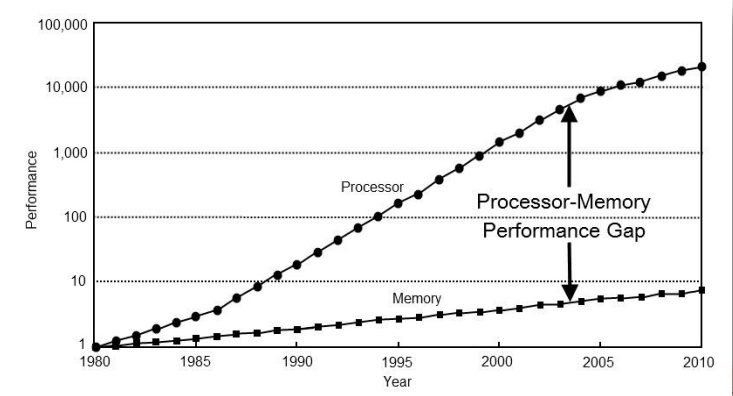
\includegraphics[width=0.7\linewidth]{PICs/cpu_memory_gap}
	\caption{"\textit{\textbf{Starting with 1980 performance as a baseline, the gap in performance
			between memory and processors is plotted over time}.
			Note that the vertical axis
			must be on a logarithmic scale to record the size of the processor-DRAM performance
			gap. The memory baseline is 64 KB DRAM in 1980, with a 1.07 per year performance
			improvement in latency (see Figure 5.13 on page 313). The processor line assumes a
			1.25 improvement per year until 1986, and a 1.52 improvement until 2004, and a 1.20
			improvement thereafter}" \mcppic{hennessy}{289}}\label{cpu_memory_gap}
\end{figure}\\
To solve the issue of ever diverging CPU/memory performances (commonly referred to as the \textit{memory gap \mcp{gregory}{189}}), specifically to reduce the latency of references to main memory, smaller but significantly faster (and more expensive) memory units are placed between the CPU and the main memory. These modules are called \textit{Caches} - first named by C.J. Conti \mcp{conti}{15} in 1969. Originally cache technology was mentioned as \textit{buffers}\mcp{cragon}{15}. Not considering their complex, modern modalities and policies this is a fitting notation.\\
The basic idea behind a fast buffer interconnected between the CPU and the main memory is to create local copies of referenced data-chunks, in order to provide faster access on subsequent calls to the same \textit{AU} (Adressable Unit) as well as the ones deemed likely to be accessed soon \mcp{gregory}{191}. This principle originated in the work on \textit{Virtual Memory} \mcp{cragon}{15} and is today much more sophisticated.\\
So high speed memory actually exists in our common computer architectures, those particular components are however limited due to their cost intensity and physical barriers.

\subsection{Cache modules and types}
In today's PCs/consoles typically each CPU core has its own hierarchy of cache modules \reffigp{cache_layout}.
\begin{figure}[!htbp]
	\centering
	\includegraphics[width=0.4\linewidth]{PICs/cachelayout}
	\caption{Exemplary, simplified model of a CPU core and its several cache modules \mcppic{Drepper}{15}}\label{cache_layout}
\end{figure}
Closest to the core (on-chip) is the \textit{L1} (Level 1) cache. Accessing an AU in the  Intel i7 Processor's L1 cache for example is almost as fast as accessing it in the very CPU's registers - ~4 cycles (2.1 to 1.2 ns) \mc{levinthal}. For reference access to main RAM "\textit{can take on the order of 500 cycles[...]"} \mcp{gregory}{189}.
Another cost unrelated reason, why there is not lots of \textit{L1 D} cache is that more memory means literally more physical space is occupied. Having more cache memory equals more \textit{cache hits} \refsecp{cpucu} but as soon as the cache can not fit on-chip anymore, there is yet again additional latency. That is why the L1 and sometimes L2 cache modules are kept comparably small but on-chip. Other L3 and L4 caches are each bigger and slower than their preceding counterparts respectively, but for the most part share the same ideas slowly converging latency times to the common main memory RAM.\\
CPU cores can share one or more cache modules (usually starting with L2 or L3), effectively accessing the same local copies of data. This entails synchronization issues as the overlying smaller and faster cache-modules may not work on diverging information.\\
Modern cache hierarchies include data caches as well as instruction caches, usually both in an L1 cache. However there are different takes on how to implement this. Harvey G. Cragon lists \mcp{cragon}{17}:
\begin{itemize}
	\item instruction cache - holds only instructions
	\item data cache - holds only the data stream
	\item unified cache - holds both instructions and data
	\item split cache - two-cache system, one for instructions and one for data
\end{itemize}
While optimizing against better instruction cache utilization can result in significant performance boosts \refsecp{conclusion}, the scope of this masters thesis will omit instruction-cache related subjects, because the upcoming attempts and techniques to achieve performance optimizations will focus on improving the data layout of a given target source code.
%local  L1 CACHE hit,                              ~4 cycles (   2.1 -  1.2 ns )
%local  L2 CACHE hit,                             ~10 cycles (   5.3 -  3.0 ns )
%local  L3 CACHE hit, line unshared               ~40 cycles (  21.4 - 12.0 ns )
%local  L3 CACHE hit, shared line in another core ~65 cycles (  34.8 - 19.5 ns )
%local  L3 CACHE hit, modified in another core    ~75 cycles (  40.2 - 22.5 ns )
%remote L3 CACHE (Ref: Fig.1 [Pg. 5])        ~100-300 cycles ( 160.7 - 30.0 ns )

\subsection{The CPUs cache utilization}\label{cpucu}
A programmer will rarely ever directly interact with a cache module (though there are mechanisms for manual prefetching/clearing). The underlying idea for it was to be transparent to the programmer. However understanding the CPUs cache utilization enables one to tailor the data layout to it, resulting in faster access, less waiting and consequently higher throughput. Among other things, this is what \textit{Data oriented Design} aims to do - developing against hardware concerns. \mcp{fabian}{268}\\
As mentioned before the basic idea of the cache is to provide local copies of data at a faster rate and prefetch data segments, that are likely to be used soon. This works by directing each main memory access to go through the cache. Main memory access means also going through virtual address translation, address and data buses and depending on the main memory, crossbar switching logic \mcp{gregory}{190}.  
Whenever the CPU requests access to a certain AU before saddling the horses and going on a journey to main memory, the cache will check whether or not the requested AU is currently present inside its buffer. If so it is referred to as a \textit{cache hit}, otherwise a \textit{cache miss}. For a modern L1 D cache this buffer, to be more specific, consists of several cache lines usually each of 64 bytes. Overall cache- and line sizes vary between different architectures and levels but are standardized mostly due to Intel's designs.\\
Cache misses result in higher access latency and should be avoided if possible. It is however not always possible. \textit{Mark Donald Hill} describes three classifications for cache misses \mcp{hill}{50}:
\begin{itemize}
	\item Compulsory Miss - Access to previously unreferenced data blocks. E.g. the very first data access will inevitably result in a main memory access.
	\item Conflict Miss - Due to data blocks mapping to the same cache-lines.
	\item Capacity Miss - Due to the cache's finite capacity. Lots of data accesses will eventually displace older/less-used entries in the cache (depending on Replacement policies).
\end{itemize}
The simplest and least efficient implementation to determine a cache \textit{hit/miss} is to iterate each cache line comparing fitting criteria. To prevent this nowadays caches implement a certain associativity technique. This way each individual physical main memory address can be mapped to one or more specific cache lines. Doing so addresses are converted to and managed by metadata consisting of: \mcp{gregory}{193}
\begin{itemize}
	\item Offset - Offset to the actual referenced Byte inside the cache line.
	\item Cache Line Index - Which cache line/s would hold the AU.
	\item Tag - Which cache sized block in main memory holds the original data.
\end{itemize}
In the case that each physical main memory address has exactly one counterpart it is called a \textit{direct-mapped} cache \mcp{gregory}{194}. In this case since the cache can by far not encompass the whole extend of the main memory, a lot of physical addresses will be mapped to the very same cache line, effectively extruding each other out of the cache when accessed. This is called \textit{eviction} and in unlucky cases will behave like all references are cache misses \mcp{cragon}{97}. To prevent this modern caches map a physical address to \textit{n} cache lines. This is described as \textit{n-way associativity} - typically implemented as \textit{8-way} or \textit{16-way} caches depending on the level.\\
There is a lot more to cover about caching technologies and policies like: Replacement-/Write-/Coherency(MESI; MOESI; MESIF) policies and for further reading Harvey G. Cragon's \textit{Memory Systems and Pipelined Processors}\mc{cragon} as well as Jason Gregory's \textit{Game Engine Architecture}\mc{gregory} are highly recommended. However for the purpose of this work a few specifics are most interesting.\\
How can a data layout affect \textit{hit ratios} and reduce calls to main memory? As mentioned before there are common data access patterns in software and the caches actually accommodate us by adapting their builtin prefetching mechanisms to it, following a set of \textit{locality concepts}. Harvey G. Cragon counts three of those concepts: \mcp{cragon}{16}
\begin{itemize}
	\item \textit{Temporal locality} - Information recently referenced by a program is likely to be used again soon.
	\item \textit{Spatial locality} - Portions of the address space near the current locus of reference are likely to be referenced in the near future.
	\item \textit{Sequential locality} - A special case of spatial locality in which the address of the next AU will be the immediate successor of the present one.
\end{itemize}
At first glance these concepts are very straight forward, but their respective implementations for automatic hardware prefetching can be more complex than one would think. Prefetching data basically means:
\begin{quote}
"\textit{[...] bringing data in the data (or mixed instruction-data) cache before it is directly accessed by a memory instruction [...].}" \mcp{chen}{610}
\end{quote}
There are however different strategies to decide which bytes should be faithfully loaded into the cache. Tien-Fu Chen and Jean-Loup Baer list two categories for prefetching strategies: \mcp{chen}{610}
\begin{itemize}
	\item \textit{Spatial} - access to current block is basis for prefetching.
	\item \textit{Temporal} - lookahead decoding of instruction stream is implied.
\end{itemize}
There are simple approaches like: whenever block \textit{i} is accessed, prefetch block \textit{i}+1, called the \textit{One Block Lookahead}; stride based approaches storing previously referenced addresses in a table and calculating a stride based on current and previous addresses; combinations of both and many more \mc{chen}.  Sometimes data is prefetched into the cache, sometimes into separate stream buffers. There are many different hardware prefetching methods to find and while data cache prefetching is considered to be more challanging \mcp{mittal}{4} it is still best practice to rely on spatial locality when modeling data to play into the cache's hand.\\
Compilers already make use of software prefetching (manual cache interaction instructions) in certain cases.
\begin{quote}
	\textit{For array-based applications, the compiler can use locality analysis to predict which dynamic references to prefetch, and loop splitting and software pipelining to schedule prefetches.} \mcp{luk}{223}
\end{quote}
So we can already deduce that for an efficient data layout it would be beneficial to rely on arrays, or more generally, concepts compilers can 'comprehend' and optimize. Also even though the concept of \textit{sequential locality} is only a special case, it is the one we can utilize best to derive adaptations for our data layout, since hardware prefetching has adapted best to it. DoD converts this information into a generic set of rules/best practices, a methodology for efficiency.

\section{Data Oriented Design}\label{dod}
The whole purpose of adding abstraction layers is moving further away from the hardware mentally. This helps us to focus on constructing appropriate models for a problem \mcp{kramer}{5}. However disregarding intrinsic detail is predestined to result in poor resource utilization at that level. \textit{Data oriented Design} wants us to be aware of what is beneath the source code and tailor the essential resources to it. Essential resources here being our data. 
\begin{quote}
	\textit{The data-oriented design approach doesn't build the real-world problem into the code. This could be seen as a failing [...] by veteran object-oriented developers [...]. [It] gives up some of the human readability [...], but stops the machine from having to handle human concepts [...].} \mcp{fabian}{7}
\end{quote}
\subsection{OOP and bad abstraction}\label{oop_bad_abstraction}
DoD however deserves more credit than only being a performance optimization. (Wrong) abstraction not only moves us away further from the hardware, but also from the actual problem domain.\\
Even though \textit{coupling} and its avoidance are a big deal in OOP it somehow seems natural to couple the data and the problem domain. This coupling has proven to lead to the exact same problems as coupling of unrelated classes. Its hard to make changes, especially when the reason for change is modification of fundamental design choices. But not only is contextual linkage rigid to conceptual change but its also hard to operate on it only in ways that haven't been thought of initially.\\
Imagine for example a simple particle system implemented in a typically OOP manner \refcodep{particle_system}.

 \begin{lstlisting}[language=C++,name={ OOP typical, simplified particle system implementation},label={particle_system}]
struct particle
{
	float ms_alive, lifetime_in_ms, xyz[3];
	Shader *shader;
};

struct particle_system
{
	particle particles[1024];
	unsigned particles_alive;
	...
};
\end{lstlisting}
At first glance it appears to be a perfectly valid approach to make a particle system linked directly to the very particles it is supposed to manage (\refcode{particle_system} line 10). Each method will now operate on the particles array and just like that we can make numerous particle systems, each implicitly operating only on its own data. This is an easy to grasp concept that in terms of a particle system we could easily match with a real-world fireworks battery. In regards of maintainability there is already a huge issue.\\
Concerning operations, that need to be applied to all particles right now this implementation does not provide an easy solution to do so. When in the real world do two physically different particle systems ever interact with each other? Collision might come to mind. While it would be a lot easier to just iterate a big list of particles, we don't really care. It is still relatively easy to just check each particle system's particles against another particle system \refcodep{collision}. And we will just do this for all the particle systems we have! They probably should exist somewhere in the same context anyway.\\
 \begin{lstlisting}[language=C++,name={Example code how OOP could handle collision between different particle systems' particles},label={collision}]
void particle_system::particle_system_collision(
	particle_system *ps1,
	particle_system *ps2)
{
	for(unsigned i = 0; i < ps1->particles_alive; ++i)
	{
		particle *p1 = &ps1->particles[i];
		for(unsigned o = (ps1 == ps2 ? i+1 : 0); o < ps2->particles_alive; ++o)
		{
			particle *p2 = &ps2->particles[o];
			[collision code]
		}
	}
}
\end{lstlisting}
Even though \refcode{collision} has some uncomfortable specifics (especially line 8), it is still doable. The moment we start to render this particle system however one might notice that the particles are occasionally blurry. The particles' sprites make use of transparency and even though transparency is enabled in the render back-end it doesn't look right. For transparency to be applied correctly,the particles need to be rendered in a certain order. This circumstance might have not occurred to the programmer while designing the data model. It is easy enough to sort one particle system's particles according to their distance to camera respectively, but bringing EACH particle system's particles in order?\\
One could write an algorithm, that has a list of particle arrays; takes each particle system's particle array; unifies them to a big dynamically allocated array; then sorts it; then returns that array so it can be rendered. Each frame. This also implies changing the render pass, since now it is not the particle systems to render but one big array of particles.\\
These changes are starting to proliferate really fast. One does not have those sort of issues with a real-world fireworks battery and might feel betrayed by the abstraction to it. Ultimately we come to a point where we understand, that a real-world projection of a problem domain into source code might not be the best choice. Its definitely possible, but does not provide the optimal attempts to solve the problems specific to certain tasks. So instead of realizing overly complex solutions to make our code fit our abstraction we realize that our abstraction is obsolete and we should focus on a solution that fits our tasks. In the end data is not generic in the way it is used\mcp{fabian}{15}. Different jobs might require different solutions and OOP might be optimal for a subset of problems, but has evolved into a pattern, that is forced on domains as a go to.\\
Besides additional layers of abstraction do not equal superior usability/readability either. When using a third party library we hope the API designer provides functions that operate on data types we are already familiar with, like char pointers, instead of forcing us to learn how to use that developers self-made string class (KISS).\\\\
So arguably Object Oriented Programming is not automatically superior, neither in terms of maintainability nor performance. Actually it appears to be inferior to DoD. So the question is: What does DoD do to be \textit{better}?\newpage
\subsection{Normalization of Data}
When thinking in terms of the problem and designing against the data \textit{Richard Fabian} references relational database models as a worthy category to look up to in his book \textit{Data-Oriented-Design: Software engineering for limited resources and short schedules} \mcp{fabian}{25}. After all a database should handle data correctly.\\
We have already seen, that the object typical data-layout makes sense in terms of readability, but fails to be maintainable and in terms of cache utilization behaves poorly. In order to peel off of the OOP abstraction pattern we want our model to be a minimal, precise representation, that abides a format, that has proven to behave well. Fabian says:
\begin{quote}
	\textit{The structure of any data is a trade-off between performance, readability, maintenance, future proofing, extendibility, and reuse.} \mcp{fabian}{28}
\end{quote}
Therefore we could attempt to treat our data modeling process the way we would, when setting up a relational database. We normalize our data, according to the existing normalization stages developed by Edgar F. Codd and Raymond F. Boyce \mc{codd}. This is done because laying out your data in a linear fashion goes away from embedding meaning to its structure (Class/Struct) \mcp{fabian}{25} and has proven to give advantageous insights to the data, its domain and the relations between its subsets. Dealing with the problem's domain and the underlying data eventually led to technologies like JPEG and MP3 \mcp{fabian}{47}. Understanding the data will lead to an understanding of the solution.
\begin{table}[H]
	\centering
	\scalebox{0.7}{
	\begin{tabular}{@{}lllllll@{}}
	\toprule
	\textbf{particle\_id} & \textbf{shader\_id} & ms\_alive & lifetime\_in\_ms & x   & y    & z     \\ \midrule
	p0                    & s0         & 7034      & 10000            & 4.0 & 10.1 & -12.9 \\
	p1                    & s0         & 122       & 10000            & 0.5 & -8.1 & -2.6  \\
	p2                    & s0         & 4310      & 10000            & 1.1 & 7.4  & -3.0  \\
	...                   &            &           &                  &     &      &       \\
	p1024                 & s1         & 86        & 100              & 7.0 & 0.0  & 0.5   \\
	p1025                 & s1         & 44        & 100              & 3.0 & 0.0  & 0.2   \\
	... &&&&&& \\
	\bottomrule
	\end{tabular}}
\end{table}
\begin{table}[H]
	\parbox{0.5\linewidth}{
		\centering
		\scalebox{0.7}{
		\begin{tabular}{@{}cll@{}}
			\toprule
			\textbf{system\_id} & particles\_alive\\ \midrule
			ps0                 & 462                   \\
			ps1					& 99				   \\ \bottomrule
		\end{tabular}}
	}	
	\parbox{0.5\linewidth}{
		\centering
		\scalebox{0.7}{
		\begin{tabular}{@{}cll@{}}
			\toprule
			\textbf{system\_id} & \textbf{particle\_id}\\ \midrule
			ps0                 & p0                   \\
			ps0                 & p1                   \\
			ps0                 & p2                   \\
			...                 &                      \\
			ps1					& p1024				   \\
			ps1					& p1025				   \\
			... & & \\ \bottomrule
		\end{tabular}}
	}

	\caption{Example excerpt of a possible first normalization step for the particle system and how it indicates bad design}
	\label{normalized_ps}
\end{table}
For our minimal example of a particle system, even just the first stages of normalization teaches us, that there should be no arrays of data in one element \mcp{fabian}{37} it also forces us to reconsider which data is accessed through which instance (key) and therefore whether or not there is a \textit{relation} to find \reftablep{normalized_ps}.\\We will not implement a relational database for our application but generating this model can help us realize some things.
\begin{enumerate}
	\item particles are no longer represented block-wise, but are held in ONE unified table to begin with.
	\item Instead of holding an array of particles we can just as well take its data subsets and link them against a unique key, which basically translates to each member is a column/array and each instance of a particle or particle system is now a mere index.
	\item There is tons of redundancy. Not logical but contextual. Seeing the same \textit{shader\_id} and \textit{lifetime\_in\_ms} over and over for each particle that will share a particle system certainly \textit{smells} funny. It is very important to be able to link each particle to a specific shader, but contextually this is redundant. We can see, that some things might have been coupled due to our abstraction.
	\item Especially after resolving redundancy, rethinking which data belongs to which entity hints at \textit{when} specific subsets are accessed and in which context (which key is used to get it) encouraging us to implement domain wise processing of an entities attributes.
\end{enumerate}
After \textit{laying out our data} in a linear fashion, we can now implement a \textit{data layout} that implements our new ideas.

\subsection{Structure of Arrays / SOA}\label{soa}
In contrast to the previously mentioned AOS \refsecp{OOP} a \textit{Structure of Arrays} (SOA) is the \textit{column-oriented database} pendant to a data layout that results in higher throughput by providing a cache friendlier structure \mcp{fabian}{163}. We already know now, that the hardware, specifically the cache uses certain strategies to provide data out of main memory, that is likely to be used soon. This happens both when loading data in cache-line sized blocks and through prefetching mechanisms \refsecp{cpucu}. Now when implementing the column-oriented approach that comes with data normalization we automatically almost perfectly conform to those auxiliary means by implementing columns as arrays. The original concept of an \textit{object} can now be simplified to an index, that retrieves the respective values in each column/array.\newpage
\subsubsection{AOS in the cache}
\begin{wrapfigure}[11]{r}{.35\textwidth}
\vspace{-1cm}
\begin{lstlisting}[language=C++,numbers=none,name={NPC pod after derivation is done},label={post_deriv_npc}]
struct NPC 
{
	//inherited from Obj 
	float xyz[3];
	float vel[3];
	//inherited from Human
	char *name;
	int age;
	//NPC
	int mood;
};
\end{lstlisting}
\end{wrapfigure}
Remembering \refcode{pods}, when examining the NPC class we know that after derivation (done by the compiler) it looks like \refcode{post_deriv_npc}. Accessing subsets of an instance of NPC will always result in loading at least a whole cache line. Let us assume, that the game code will iterate over the NPCs to update their positions by adding their velocity multiplied with a delta-time to their current xyz. With a typical L1 D cache-line of 64 Byte and assuming that an NPC is 40 Byte (float = 4 Byte, pointer = 8 Byte) we can make the following assumptions: Considering the subset of data we actually want to work with on our update routine per NPC is $2\times 3\times \textit{sizeof(float)} = $ 24 Byte, we waste $40 - 24 =$ 16 Byte of our cache per NPC. Due to our algorithms complexity \refsecp{asymptotic_notations} this waste scales linearly with our data.\\
As a quick approximation onto a damage report we could do the following:
The smallest common multiple of our 40 Byte NPC and our 64 Byte cache-line is 320, so with eight NPCs we load five cache-lines \reffigp{cache_utilization_npc}. This equals five compulsory misses. After 320 Byte this layout repeats so we could extrapolate to greater numbers of NPCs \reffig{soa_aos_cl_usage}. 
\begin{figure}[!htbp]
	\centering
	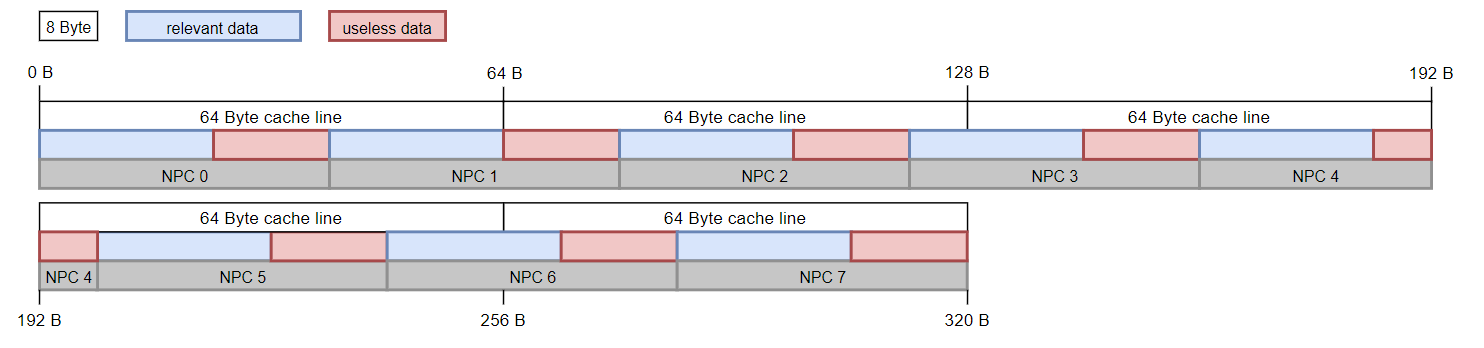
\includegraphics[width=1.0\linewidth, height=0.3\linewidth]{PICs/CacheUtilizationNPC}
	\caption{NPCs inside cache-lines, where blue is relevant data and red blocks represent unused data}\label{cache_utilization_npc}
\end{figure}
A cache miss occurs whenever we do not find an AU inside a cache line. While \textit{NPC0} completely fits inside the first cache-line, \textit{NPC1} does not. However \textit{NPC1}'s relevant data also completely fits in the first cache-line, so accessing it's relevant data will not result in a cache miss! While accessing \textit{NPC2}'s relevant data will partly load \textit{NPC3}'s relevant data, we will only get the first eight Byte of it. The remnant will be loaded separately, yet this will result in completely loading \textit{NPC4}'s relevant data.\\
Continuing this we will count five cache misses and foregoing from 320 loaded Bytes this process will repeat. The statement that 1000 NPCs will count $1000 npc = \frac{5 * 1000}{8} cms = 625 cms
$ cache misses for the position update routines (where \textit{cms} are cache misses), is only a narrow assumption, since our cache-lines are defined in fixed quantums \reffigp{soa_aos_cl_usage}.
\subsubsection{SOA in the cache}
\begin{wrapfigure}[9]{r}{0.4\textwidth}
\begin{lstlisting}[language=C++,numbers=none,name={SOA variant of the NPC},label={soa_npc}]
struct NPCs{
	float xyz[3 * NUM_ENTITIES];
	float vel[3 * NUM_ENTITIES];
	char *name[NUM_ENTITIES];
	int age[NUM_ENTITIES];
	int mood[NUM_ENTITIES];
} npcs;
\end{lstlisting}
\end{wrapfigure}
Implementing the \textit{NPC} in a SOA manner it could look like \refcode{soa_npc}. What used to be individual class members are now columns/arrays, accessed by a key - the \textit{npc\_id}. From now on both reads to \textit{xyz} and \textit{vel} will fill a cacheline worth of relevant data, respectively. A single cache-line now holds up to five ($5\frac{1}{3}$) positions or velocities. This doesn't prevent our data from overlapping in terms of cache-lines. The smallest common multiple of 12 and 64 is 192, so over $\frac{192}{64}=3$ cache-lines we will fit $\frac{192}{12}=16$ units. As can be seen in \reffig{soa_aos_cl_usage} the SOA attempt will develop better cache utilization for contiguous AU access on rising data sizes, disregarding any external eviction. This does not automatically equal the amount of cache misses, since repeated data access will find the data in the cache. But a SOA data model will reduce compulsory misses.
\subsubsection{}
\vspace{-1cm}
\begin{wrapfigure}[16]{l}{.6\textwidth}
	\centering
	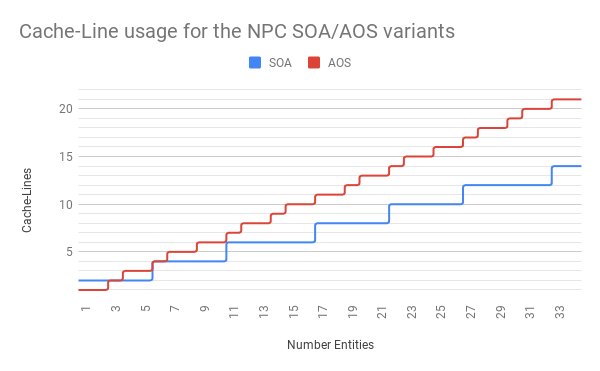
\includegraphics[width=.6\textwidth, height=0.42\textwidth]{PICs/soa_aos_cl_usage}
	\caption{Cache-line efficiency comparing NPCs represented as SOA and AOS.}\label{soa_aos_cl_usage}
\end{wrapfigure}
The unit we use for computations here is the size of three floats (12 Byte), so while a cache-line fits $\myfloor{\frac{64}{12}}=5$ complete units, the remnant of $64-12\times5 = 4$ Byte will belong to a unit, we will need another cache-line for. This overlap happens exactly $\frac{12}{64-60} = 3$ times until in the fourth cache-line this process repeats. Distributing logically dependent data over multiple cache-lines should be avoided, since access to it will result in more cache misses and is prone to eviction \mcp{intel}{12-19}.\\
It can be solved by adjusting the data's \textit{alignment}. Since this will be used in the prototypical implementation it will be explained in section \ref{memory_management}, for now we could assume, that we align and pad our \textit{float[3]} blocks of data to our cache-lines in a way that each cache-line holds exactly five of those entities \reffigp{cache_utilization_soa}.\\
This leads to consistent throughput. In numbers we now have exactly two cache misses per five \textit{NPCs} (We don't really have an NPC object anymore, but we are still allowed to \textit{think} in objects). One for the positional data, one for the velocity data. Again for 1000 NPCs this would now result in 400 cache misses what translates to $225\times\sim300$ clock cycles less latency than the AOS version, for position updates alone! Each frame!
\begin{figure}[!htbp]
	\centering
	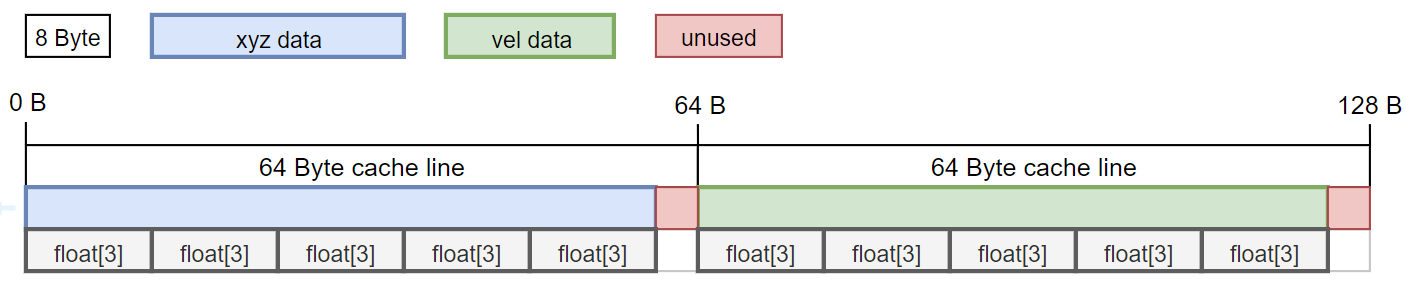
\includegraphics[width=1.0\linewidth, height=0.17\linewidth]{PICs/CacheUtilizationNPCSOA}
	\caption{xyz and vel blocks inside cache-lines, where blue represents joint float[3] blocks of xyz data, green joint blocks of float[3] vel data and red is unused but intentional padding.}\label{cache_utilization_soa}
\end{figure}
This is starting to behave \textit{optimal}. By not loading unneeded data into the cache we can store more relevant data. By Aligning and padding our data blocks correctly we attenuate the chance of \textit{conflict misses} since we reduce the number of cache-lines the related data depends on. We do however still have leftover space. The four Byte paddings we append to each $5\times float[3]$ block has purpose, yet could theoretically hold information. Imagine our now theoretical NPC and thus our positional computation would involve a per NPC factor for maybe damping, as well as a mass. Still assuming that $sizeof(float) = 4$ this would be an additional eight Byte per NPC on each computation. Following our SOA approach we would define yet two new arrays for the damping factor and mass respectively. Accessing them would result in the utilization of another two cache-lines. Even though those cache-lines now suffice 16 NPCs each ($\frac{64}{sizeof(float)} = 16$) we now are dependent on four individual cache-lines to compute the \textit{update\_npc\_position} for one NPC, so the amount of cache-lines scales linearly with the amount of parameters the computation depends on (for SOA). In terms of eviction and consequently of conflict misses, this could yet again cultivate sub-optimal cache utilization (for the same reasons Intel's article on \textit{Memory Layout Transformations} \mc{aosoa} also mentions increased pressure on the \textit{TLB} (Translation Look-aside Buffer)). Even though we reduced the overall NPC per cache-line ratio, there is still unused information and scaling prone to eviction, all due to the individually related data blocks being physically separated. This doesn't countermand that SOA performs better than AOS, but it indicates that it might only be optimal for certain types of computations (e.g. SIMD) there is still room for improvement.\\\\
Note that while SOA greatly fits SIMD it is not considered to be an ideal solution to encompass objects \mcp{gregory}{1060}. For that we need solutions, that regard both temporal and spatial locality. 

\subsection{Regarding temporal- and spatial locality}\label{rtasl}
The motivation behind our AOS to SOA conversion, was to maximize cache utilization when processing an NPC's position. We figured, that loading an object entails lots of unwanted data that does not share temporal locality with the information that is relevant to us. So we made sure, that instead of objects we loaded only wanted data.
\begin{wrapfigure}[10]{r}{0.4\textwidth}
\begin{lstlisting}[language=C++,numbers=none,name={Consolidating related data},label={component_npc}]
struct npc_group{
	float xyz[3];
	float vel[3];
	float mass, damping;
};

npc_group npc_groups[NUM_ENTITIES];
\end{lstlisting}
\end{wrapfigure}
In order to do so we gave up something very important. When data is logically related it means, that it collaborates/is involved in the same data transformations. Whenever we see, that certain subsets of data are frequently used together it is advisable not to separate them. So instead of rigorously converting each member into an array pendant, we group logically related data and create arrays of those groups instead \refcodep{component_npc}.This way the relevant data concerning one NPC will not spread over different incoherent cache-lines, that could map to completely different segments in main memory.\\\\
This technique bundles related data and makes sure it is successive in memory as well as in cache-lines, consequently we won't peril those cache-lines to extrude each other from the 
\subsubsection{}
\vspace{-1cm}
\begin{wrapfigure}[8]{l}{0.37\textwidth}
	\vspace{-0.4cm}
	\centering
	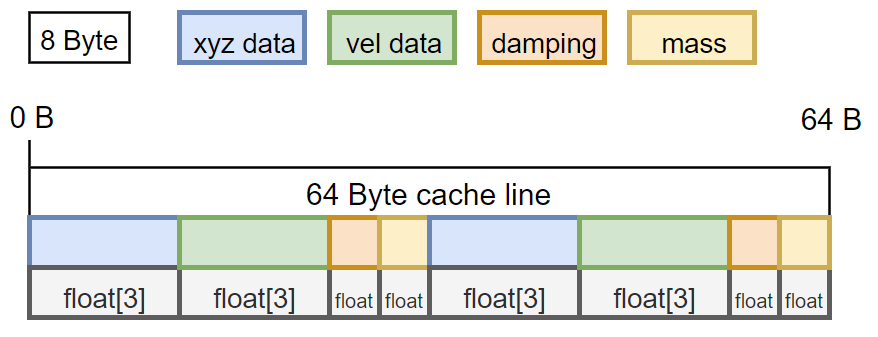
\includegraphics[width=.37\textwidth, height=0.17\textwidth]{PICs/CacheUtilizationNPCComp}
	\caption{Unified/Grouped relevant data in a cache-line.}\label{cache_utilization_comp}
\end{wrapfigure}
cache. The book \textit{Compilers, Principles, Techniques and Tool} also describes a mechanism like this and refers to those groups as \textit{blocks} \mcp{aho}{786}.
Also we get the chance to fully exploit our hardware's boundaries, as in now we can get rid of manually inserted padding Bytes \reffigp{cache_utilization_comp} - provided we have related data that fits the gap. It is however only possible to gain a performance boost out of this, when the unified data shares temporal locality.

\subsubsection{Hot/Cold Splitting}\label{hot_cold_splitting}
\begin{wrapfigure}[15]{r}{0.3\textwidth}
\begin{lstlisting}[language=C++,numbers=none,name={The NPC class splitted into hot/cold data},label={hcsplit_npc}]
struct npc_cold_data{
	char *name;
	int age;
	int mood;
};

struct npc{
	float xyz[3];
	float vel[3];
	npc_cold_data *cold_data_ptr;
};
\end{lstlisting}
\end{wrapfigure}
A famous practical application of grouping a particular subset of data is called a \textit{Hot/Cold Split} \mcp{nystrom}{283}. It is also used to improve cache utilization, it only has a very specific definition of what members should be grouped.\\
The idea is to separate a record's member definitions into two subsets. One that contains all the hot-, and one that contains all the cold members respectively. Data is hot when it is used frequently and cold when it is used rarely \mcp{chilimbi}{8}. By grouping together all the hot data we want to make sure, that data which is frequently used has a higher chance to exist in a cache line on access.\\
The cold data is externalized into a struct of its own. The original struct now contains only the hot data, as well as a pointer to a cold struct instance. Since access frequency does not necessarily resemble the original partitioning of the fields, this pattern emphasizes the preference of logical over contextual relation.\\
Especially for monolithic class definitions, there can be numerous logical subsets of data fields. For example one data subset of a classic OOP gameobject will mainly be used for physics calculations (velocity, acceleration, mass, colliders), another for rendering (vertice data, shaders, textures) and yet another that embeds the game object in the game's environment (health, strength, gold, stamina, etc.).\\
First of all it is not always apparent whether a field is hot/cold. An experienced programmer might feel confident enough for a reasonably small class definition to eyeball it. A better approach might be to wrap our fields with access mechanisms that let us count how often they are accessed at run time, yet again we could rely on static analysis. Since this work will specifically implement a prototypical tool that performs automated hot/cold splits we will discuss this further in \refsec{prototype}.\\
Also we might end up picking individual fields of contextually differing data subsets. We could for example identify \textit{velocity, vertice data, gold} as our hot fields, because they are frequently accessed. However they are utilized at different times of the game and individually they have no common logical relation that is relevant to our computations! Access frequency ca not be the sole deciding factor for a split so this pattern should only be applied when a certain knowledge about underlying hardware components is given.\\
Whenever we split a record we reduce both the size of the hot data and the stride to get to subsequent instances resulting in better cache utilization \reffigp{memory_mountain}. So in terms of a heuristic (that we will later describe) we want to cutoff as much fields as possible.
\begin{figure}[!htbp]
	\centering
	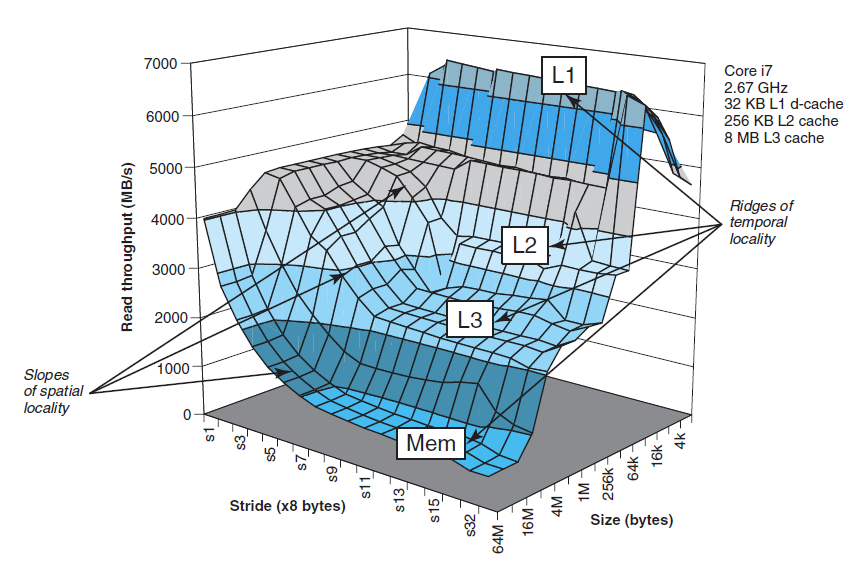
\includegraphics[width=\textwidth, height=0.5\textwidth]{PICs/memory_mountain}
	\caption{Relation of a record's stride and size to the read throughput, characterized as the memory mountain. \mcppic{bryant}{623}}\label{memory_mountain}
\end{figure}
Even a split that divides contextual relation might result in a performance boost, if only the cold data is 'cold enough', but just as well a bad split might result in even worse cache utilization.
In order to make a decision, that regards temporal- and spatial locality in a complex situation, we might need to find a way to evaluate, compare and eventually prioritize individual fields. An attempt to solve this will be made in the prototypical implementation, so more on that later on in \refsec{prototype}.

\subsubsection{Components}
After a grouping procedure the remnant members of the original NPC class could also be grouped by the same method that was mentioned before: take related members unify them in a struct and store those structs in an array in order to create spatial locality for domain related data. If the original class hierarchy was designed well in terms of cohesion metrics, the grouping of related data bits will start to resemble it, which might look like a step backwards at first, but remember, the related data groups are packed in seperate single purpose arrays and what counts is the access patterns to retrieve them. When we are done grouping all related data bits of the original NPC object, we will have recreated a so called \textit{component pattern} \mcp{nystrom}{213}.\\
In the classical component pattern we will keep a container object that holds instances of each component \mcp{nystrom}{214}. In favor of performance the container object should only hold pointers to the instances lying in their respective array. But actually and if we were able to group all members of the original class, the object might be nothing else but an index, that can be used to retrieve a group out of its array.\\
Components are one widely used mechanism to decouple parts of a formerly shared entity. This is applied to classes and is therefore a statement to how OOP and DoD can work hand in hand. Not only is the component pattern useful for decoupling and performance interests, it also solves issues, that would normally be solved by applying multiple inheritance \mcp{nystrom}{215}, which is a practice often despised even by OOP enthusiasts.\\
Components can be stored domain wise, while still being contextually linked individually on an object instance level. Their decoupling mechanism has proven great maintainability and even provides a comparably light weight interface for game designers. Accessing them can be done domain wise as well -> optimal cache utilization. This elegant arrangement between OOP and DoD makes it a favored pattern for modern game engines \mcp{fabian}{83}.
\subsubsection{Array Of Structure Of Arrays (AOSOA)}\label{aosoa}
\begin{wrapfigure}[9]{r}{0.4\textwidth}
\vspace{-1.4cm}
\begin{lstlisting}[language=C++,numbers=none,name={AOSOA variant of grouped NPC traits},label={aosoa_npc}]
struct npc_bucket{
	float
	xyz[3] [SUB_SET_SIZE],
	vel[3] [SUB_SET_SIZE],
	mass   [SUB_SET_SIZE],
	damping[SUB_SET_SIZE];
};

npc_bucket npc_buckets[NUM_BUCKETS];
\end{lstlisting}
\end{wrapfigure}
At first glance the idea of reintroducing the AOS concept seems confusing. In some cases depending on the original access patterns it might however be a good idea to separate the total amount of data into chunks that are often referred to as \textit{Buckets} or \textit{Tiles}. We already went a step back before, when we decided to unify logically related bits and make arrays of groups. We figured, that this might be an optimal solution for a very specific computation, but might behave poorly in other situations. Whenever data is grouped we might have the same problem, we tried to get rid of in the first place - possibly loading unwanted data into the cache, increasing access latency. The moment we decide, that for example our game should play a scary sound when the players distance to an NPC falls below a certain threshold, we again would be doomed to load adherent information about the NPC's velocity, mass and stuff that was grouped to make position updates faster. Because for this we actually only want the NPCs' positions.\\
An attempt to solve this, is to yet again separate the relevant members, however to a certain extend gain back the advantage of spatial locality. Applied to our NPC it might look like \refcode{aosoa_npc}. We merely define our former \textit{columns}/arrays to hold only a subset of the total data respectively. The structures, that hold our member-arrays (the SOA) will however now be emplaced inside an array itself (the AO)! In Other words: We keep the data that will be used to transform each other close to prevent eviction. We enable the user to access specific subsets individually, to prevent/appease loading unnecessary information. \textit{The idea here is to get the benefit of locality at the outer-level and also unit-stride at the innermost-level} \mc{aosoa}. This attempt is compossible with grouping certain members, too. After all we are still able to access only specific sub arrays of buckets. A bucket should consist of logically related data, so we know that for a bucket's member array $a_{n}$ and an element index $npc_{e}$ each member array $a_{0\dotsc n-1}$ of a bucket contains data that is relevant to a distinct set of computations at position $npc_{e}$. For example $npc\_buckets[0].xyz[1]$ and $npc\_buckets[0].vel[1]$ will contribute to a distinct computation since they are used to describe a single abstract entity's state.\\
Finding the NPC nearest to the player would now mean iterating the \textit{xyz} subsets of each bucket. Depending on the data bundled in a bucket (especially concerning alignment and padding) we still need to expect to load unwanted data subsequently to \textit{xyz} but this will now happen on a \textit{per-bucket} basis rather than on a \textit{per-NPC} basis.\\\\
A crucial factor to the performance of an AOSOA data layout is its subset size and the resulting \textit{bucket-size\textbf{:}number-buckets} ratio. In case of our \refcode{aosoa_npc} example, taken to the extreme $\textit{NUM\_BUCKETS}=1$ would practically result in the classic SOA model, coming with all its advantages and disadvantages. On the other hand $\textit{SUB\_SET\_SIZE}=1$ would pretty much just be an object definition again (so AOS only needlessly more confusing and incomplete since we may have grouped the members).\\
Concerning our \textit{SUB\_SET\_SIZE}, independent of a cache's associativity, the \textit{eviction} of elements inside contiguous blocks of memory  will only ever occur when the data's size exceeds the cache's capacity (not considering other processes). One first conclusion could be, that our bucket's size should not exceed our L1 D cache capacity (e.g. 32KiB), to guarantee, that the adressable unit at $a_n + npc_e$ will not be evicted by access on $a_{n+1}+npc_e$ nor by any access on $a_t+npc_e$ where $t > n$.\\
Additionally \mcp{intel}{61} advises us to "\textit{Optimize data structures [...] to fit in one-half of the first-level cache [...]}" (e.g. 16KiB) because the cache is hardware and therefore shared by all processes currently running. We usually ca not expect exclusive access and full cache capacity exploitation. Demanding all resources might perform well in a situation where no other processes demand frequent main memory access. It might also be prone to eviction when the systems workload is increased. Multi way associativity techniques accommodate us to great amounts in this case, but the moment we are trying to utilize a cache in its entirety we foster concurrency between processes, that will eventually affect the entire system.\\
Going even further \mcp{intel}{3;66} warns about it's L2 hardware prefetching mechanisms to only work within page boundaries (e.g. 4KiB), so making sure a bucket fits this criteria we could further advance optimal prefetching behavior, because we ensure, that no $a_n+npc_e$ and $a_n+npc_{e+1}$ will exceed a page boundary. This complies to the principle of page locality \mc{aosoa}.\\
We're not even done yet. AOSOA  perfectly suffices parallelization. Dependent, on which cache level is shared among the CPUs/Cores we could further optimize against it by adapting our bucket's size to for example an L2 128 Byte cache-line, resulting in a \textit{SUB\_SET\_SIZE} of $\frac{128}{8\times sizeof(float)} = 4$, guaranteeing minimal cache-level synchronization overhead.\\
Another approach could be to determine the ratio between \textit{single-entity-access-patterns} to \textit{domain-related-access-patterns} in the source program. The more our application relies on entity-access patterns, meaning we want all or most of an entity's members (classic OOP access) the smaller our subsets could be. On the other hand, the more our application relies on domain-related access patterns, meaning we want one or a few of our entities' specific members, the greater our subsets should be.\\\\
The AOSOA pattern is highly flexible making it a fit for a lot of use cases. Its limitations are defined by the minimal bucket size and the optimization goals. The Buckets' sizes can be modified at compile time or at run time. This way even when one ca not reason about subset sizes, there is still the possibility to just try out different iterations and document changes in performance/cache utilization.


\chapter{Motivation}\label{motivation}
We have now seen some of the fundamental differences between \textit{Object Oriented Programming} and \textit{Data oriented Design}. After recognizing the existence of a \textit{memory gap} we got to know some of the memory units our modern computer architectures are composed of. This helped us understanding why the caching technologies we make use of today tolerate but do not thrive on the real world metaphors we use to design our data models.\\
We learned that DoD offers methods that comply to our modern hardware, by trading abstraction as well as readability in exchange for performance. So in terms of utilizing the memory hierarchy it is inarguable superior to OOP. But we have also identified abstraction as one of the most important concepts in programming \mcp{bryant}{24} and to be one of the most important skills a programmer can have, since it is directly linked to a humans capability to solve a problem. We came to an understanding, that the abstraction model, that OOP inherits to us is widely accepted and applied in the industry, because it is intuitive and easy to learn.\\
Even when one is ready to abandon OOP it will persist. The industry is known for its reluctance to change. Implementing a new programming language into a developer team might be beneficial in long term, but comes with less to zero temporary productivity and initial training. Also DoD requires an understanding of hardware concerns, that novices and fresh graduates might not have. Most projects and companies are not even that dependent on high performance code, instead rely on solutions, that are quickly developed and easy to maintain and for the same reasons even the games industry won't solely rely on DoD probably ever. We also depend on gameplay programmers or level designers who will interact with an engine heavily but should not have to think about the underlying hardware all the time \mcp{fabian}{260}. The point is: No matter how much better other programming paradigms are on certain viewpoints and for specific tasks, OOP has its \textit{raison d'etre}. Instead of trying to sort it out we might just try to find a way to get the best out of both worlds.

\subsubsection{The best out of both worlds}
We already determined that DoD and OOP can get along to certain extends \refsecp{rtasl}. The more we want to rely on DoD to obtain performance boosts however, the more we will dismantle our abstraction step by step. Ideally we could keep whats best about OOP and still have optimal performance as though we had implemented our idea using DoD.\\
As mentioned before in \refsec{oop_bad_abstraction} DoD is not inferior to OOP in terms of maintainability per se. DoD's greatest disadvantage is, that it doesn't allow us to transfer a problem into code, the way we perceive it in the real world. The intuitive and thus advantageous abstraction model that comes with OOP is lost. On the other hand better performance makes a strong case for DoD, especially for game developers.\\
In conclusion what we want is the real world metaphors coming with OOP as well as the performance benefits coming from a data layout, that facilitates optimal cache utilization. Still, the question on how it is possible to achieve both things, remains.

\subsection{Native language support for DoD principles / ISPC / JAI}\label{nat_lan_sup}
There are languages in existence and under development, that aim to provide native support for SOA/AOSOA data structures!

\subsubsection{Intel's ISPC}
\begin{wrapfigure}[11]{r}{0.34\textwidth}
\vspace{-0.8cm}
\begin{lstlisting}[language=C++,name={ISPC's native SOA support},morekeywords={soa}, label={ispc_npc}]
struct npc_group{
	float x, y, z;
	float v_x, v_y, v_z;
};

soa<128> npc_group pos_and_vel;
soa<16> npc_group aosoa_pos_and_vel[8];
\end{lstlisting}
\end{wrapfigure}
The \textit{Intel SPMD Program Compiler} (ISPC) is specifically designed to support quick and easy development of \textit{Single Program Multiple Data} \textit{SPMD} applications, making use of implicit \textit{Single Instruction Multiple Data} (SIMD) vector units \mc{ispc}.\\
Those instructions depend on SOA data layouts, thus the language provides a \textit{soa} keyword to automatically transform an AOS defined struct into a SOA format. In \refcode{ispc_npc} an AOS \textit{npc\_group} is defined in line 1. In line 6 the \textit{pos\_and\_vel} is defined as a SOA holding 128 consecutive \textit{x}, \textit{y}, \textit{z}, \textit{v\_x}, \textit{v\_y}, and \textit{v\_z} respectively. This also easily enables for AOSOA format as can be seen in line 7.

\subsubsection{Jonathan Blow and JAI}
\begin{wrapfigure}[6]{r}{0.34\textwidth}
\vspace{-0.8cm}
\begin{lstlisting}[language=C++,name={JAI's native SOA support},morekeywords={SOA}, label={jai_npc}]
npc_group :: struct SOA{
	xyz : [3] float;
	vel : [3] float;
};
\end{lstlisting}
\end{wrapfigure}
A prominent game developer and critic of the C++ language Jonathan Blow for example is working on the \textit{JAI} programming language. There is currently no official documentation to it and it is unknown when the language will be released to public, but some of its features and its design goals are already well known. One of the highly anticipated features is automatic AOS to SOA conversion done by the compiler using nothing but a single keyword. There is no official documentation and information presented here originates only from the various online video talks Blow provides occasionally (e.g. \textit{Making Programming less terrible} by Jonathan Blow from 2017 \mc{jonblowtalk}). In \mc{jonblow} the \textit{SOA} keyword is introduced as a typespecifier when creating a struct, automatically informing the compiler to store the struct's members in a SOA fashion and granting correct access to them \refcodep{jai_npc}.

\subsection{High level abstraction hiding DoD}
However we already know, that introducing new languages/technologies into a functioning industry is mostly viewed as a cost factor and since C++ is the most prominent language in the game development industry, we can not expect to see a lot of native language support for DoD principles like SOA in the near future (unless the ISO C++ committee decides in its favor).\\
One possible solution could be to provide high level abstraction containers, that internally work with data oriented concepts. In his online blog article \textit{Implementing a semi-automatic structure-of-arrays data container} \mc{reinalter} Stefan Reinalter introduces a possible implementation for such mechanisms. Template meta programming is a way of interacting with the compiler and can to a certain extend overcome the inherent conflict between OOP and DoD, but Reinalter states that:
\begin{quote}
	\textit{I really would like to have a fully automatic implementation, but I don’t believe that’s possible without compiler support.} \mc{reinalter}
\end{quote}
Even when we can provide high level data containers, that implement a cache friendly data layout, it can not completely decouple the process of modeling the reality into code from reflecting about its data layout considering optimal hardware utilization. The high level containers in the end still need to be used correctly and based on implementation may require to define the relevant records dependent on it (for example with macros), because due to missing \textit{reflection} features, we can't iterate a record's members.\\
If possible an ideal solution would be uncorrupted high abstraction code, that somehow translates to high performance code. The relevant keyword here is \textit{translate}. Compilers normally do these kinds of tasks. The question arises whether we could utilize compiler technology to accomplish our goal.
\chapter{Compiler technology as a mediator between OOP and DoD}
The inherent purpose of a compiler is to read a program defined in a \textit{source language} and translate it to an equivalent pendant for a \textit{target language} \mcp{aho}{1}.\\
Compilers provide some of the most important features a programmer needs, like syntactic and semantic analysis steps, which can automate the process of finding errors and even just smelly code. To do that they need some sort of 'understanding' for the program.

\section{A compiler's understanding of the program}\label{compilers_understanding}
\begin{wrapfigure}[8]{r}{0.4\textwidth}
\vspace{-0.8cm}
	\begin{lstlisting}[numbers=none, name={Exerpt of example context free grammar defining a (if)statement. Bold = terminal; italic = nonterminal}, emph={stmt, optexpr}, emphstyle=\itshape, morekeywords={expr, if}, mathescape=true, literate={->}{$\rightarrow{}$}{1}, label={bnf}]
	stmt -> expr ;
		| if ( expr ) stmt
	\end{lstlisting}
\end{wrapfigure}
Modern compilers implement several \textit{phases} bundled in \textit{passes} to provide an abstraction rich routine from reading mere character sequences until generating char sequences in the target language \reffigp{compiler_phases}. Of course compilers are not thinking entities, but there are mechanisms to formally define a language as well as steps to generate semantic statements with it, ordering them in a way so that a computer can process them in a meaningful way.
\subsubsection{Syntax definition}
\begin{wrapfigure}[10]{l}{0.32\textwidth}
	\begin{center}
		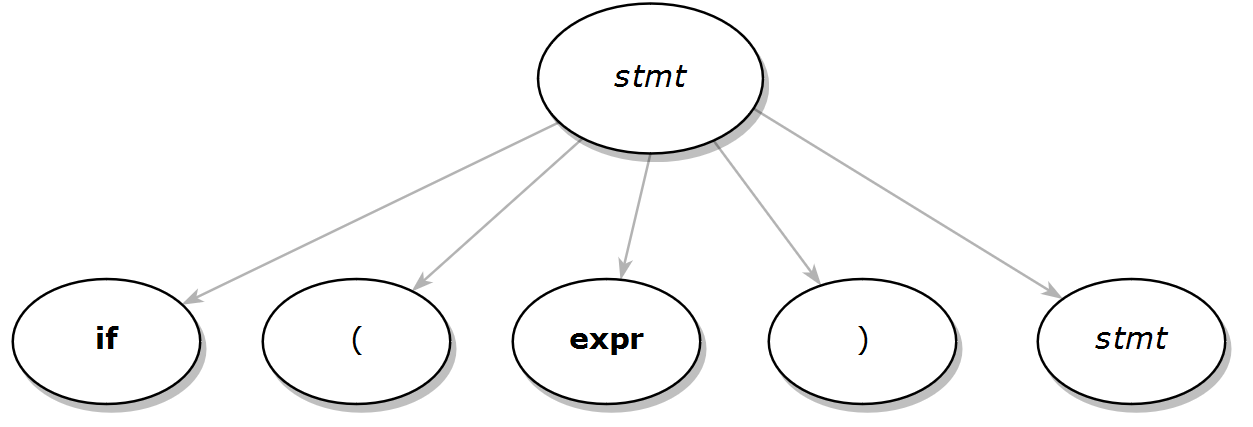
\includegraphics[width=.32\textwidth, height=0.12\textheight]{PICs/parse_tree}
	\end{center}
	\caption{Parse tree for the if-stmt node.}\label{parse_tree}
\end{wrapfigure}
\vspace{-0.5cm}
A syntactical language definition can be done using the \textit{context free grammar} notation or \textit{BNF} (Backus-Naur Form) \mcp{aho}{40}. Those grammars define a hierarchy of rules on how to form statements/expressions in the language. By defining a set of elementary symbols (\textit{terminals}) for example keywords we can then define more complex \textit{nonterminals}, like defining how a statement is formed. Ultimately we can make \textit{production} rules that describe for example our control flow statements \refcodep{bnf}. Just like this set of grammar rules basically constitutes a hierarchy, we can deduce a \textit{parse tree} for it as a concrete implementation, where beginning from the start symbol are able to derive valid successors for each symbol by iterating its child nodes. Given a statement like: "$\textit{\textbf{if} \textbf{true}) i++;}$". After reading the first token \textit{if} we can iterate our parse tree's production node for that statement and easily see, that the rule demands an opening bracket immediately following the if terminal, rendering the input as syntactically ill-formed \reffigp{parse_tree}. To be able to analyze a program like this we initially need to pass through a few \textit{phases} transforming and collecting data until we have a representation, we can work with.

\subsubsection{Lexical analysis}
\begin{wrapfigure}[20]{r}{0.2\textwidth}
\vspace{-1cm}
	\begin{center}
		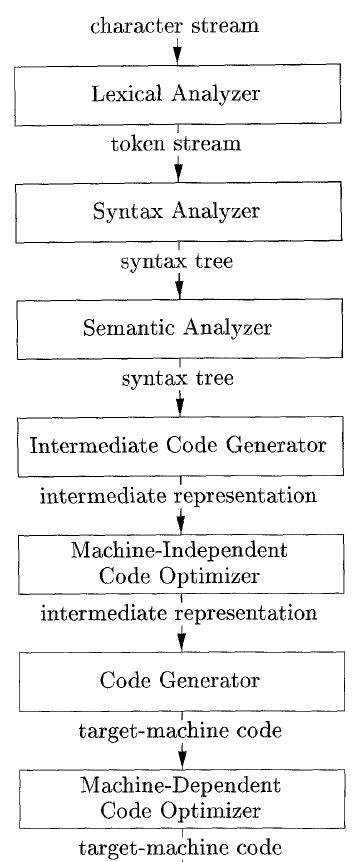
\includegraphics[width=.3\textwidth, height=0.45\textheight]{PICs/compiler_phases}
	\end{center}
	\caption{Phases of a compiler \mcppic{aho}{5}.}\label{compiler_phases}
\end{wrapfigure}
The compilers \textit{Lexer} or \textit{Scanner} takes the raw sequence of chars forming the source code and creates tokens out of char subsets it identifies as such. This information is used to fill the \textit{Symbol table}, which holds information like types, relative positions of the values, scopes and more. The symbol table is used in several following phases and essential for correct linkage of different compilation units.
\subsubsection{Syntax analysis}
The syntax analyzer creates the first \textit{Intermediate Representation} of the source code, the \textit{Syntax Tree} or \textit{Abstract Syntax Tree} (AST). It takes the token stream provided by the first phase and orders them in a tree like structure that already accounts for computational order and depicts the the grammar of the input.
\subsubsection{Semantic analysis}
Analyzing the AST from the previous phase is the \textit{Semantic Analyzer}'s duty. It traverses the AST and constantly compares its nodes with the formal language definition and gathers information like type traits. Consequently \textit{type checking} - which is important for statically typed languages - will take place in this phase \mcp{aho}{5-9}.

\section{A useful interface / LibTooling}\label{a_usfl_int}
As can be seen in \reffig{compiler_phases} there are several more phases left to describe, however \refsec{compilers_understanding} already provides information that we can utilize towards implementing a tool, that automatically translates OOP code into a cache friendly pendant.\\
Assuming we have access to our programs AST, we could start analyzing the code in an environment, that allows us to traverse the code in a tree like fashion. This means easy access to the defined data layout, as well as the access patterns in use.\\
Luckily modern compilers are designed in a modular fashion and usually define \textit{front ends} and \textit{back ends} to facilitate a multiple language to machine mapping. The front end consists of the analysis phases as well as the intermediate code generation phases for a source language. After generating an intermediate representation (IR) it is forwarded to the back end which \textit{synthesizes} the end product in the desired target language \mcp{aho}{4}.\\
The front end is especially interesting to us since it provides us with the appropriate representations to thoroughly investigate a program.

\subsubsection{LLVM/Clang}
\begin{wrapfigure}[9]{r}{0.3\textwidth}
\vspace{-20pt}
\begin{lstlisting}[language=C++,name={Example code in a Foo.cpp file},label={foo_code}]
struct Foo {
	int bar;
};

int main(){
	Foo f;
	f.bar = 10;
}
\end{lstlisting}
\end{wrapfigure}
A rather prominent representative of such an assembler/compiler/debugger tool-chain is the open source LLVM project. The front end functionality for C++ is here implemented in the Clang compiler. All the functionality is accessible and furthermore served through diverse production-grade reusable libraries and interfaces \mc{lattner} - for example the \textit{LibTooling} library that brings functionality for parsing code, creating ASTs and running \textit{FrontEndActions} over it. There are already mechanisms for recursive AST traversal like \textit{Recursive AST Visitors} and AST matching functionality with the \textit{AST Matchers}. Also tools like \textit{clang-query} provide a \textit{REPL} (Read-Eval-Print Loop) environment for quick testing.\\
In \refsec{nat_lan_sup} we saw, that languages supporting DoD natively rely on particular keywords to tag a record as SOA layouts for the compiler. We will try to carefully select the right ones using appropriate metrics (Not each record will qualify for our optimization). In case of finding any records at all it is easy enough, thanks to the functionality coming with Clang.
\begin{figure}[!htbp]
	\centering
	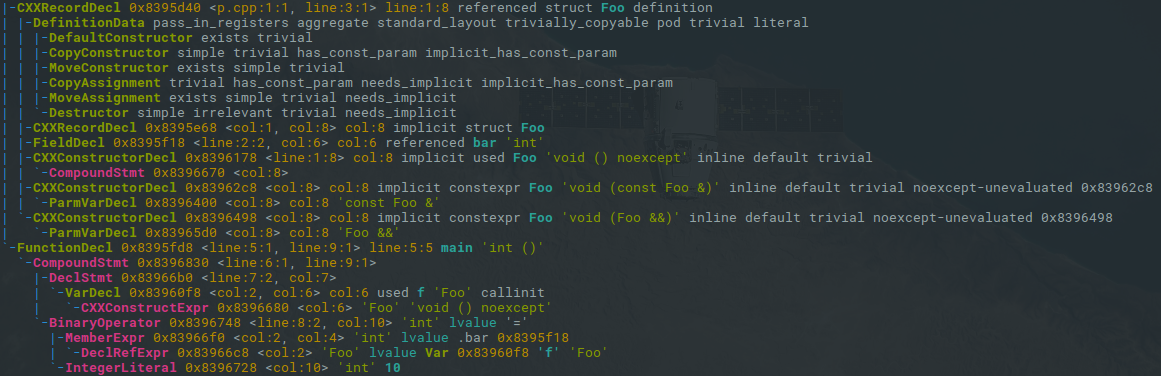
\includegraphics[width=\linewidth, height=0.5\textwidth]{PICs/foo_code_ast_dump}
	\caption{AST dump of \refcode{foo_code} generated with \textit{clang -Xclang -ast-dump Foo.cpp}.}\label{foo_code_ast_dump}
\end{figure}
The \textit{AST Matchers} and the online \textit{AST Matcher Reference} offer an excellent modular way of matching AST nodes against predefined patterns. Working with an AST is of course a lot more comfortable than working on plain text, but it also entails a new domain that one needs to familiarize with. Clang also provides proper functionality to do so. For example seeing what kind of AST nodes there are in a certain source code. When using \textit{'clang -Xclang -ast-dump Foo.cpp'} on \refcode{foo_code} among additional meta information we will see something like \reffig{foo_code_ast_dump}.
\vspace{-0.9cm}
\subsubsection{}
\begin{wrapfigure}[23]{l}{0.5\linewidth}
	\centering
	\vspace{-20pt}
	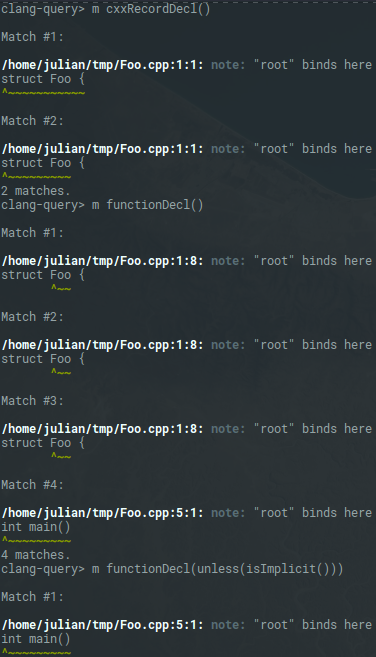
\includegraphics[width=\linewidth, height=0.7\textwidth]{PICs/clang_query_foo_code}
	\caption{AST dump of \refcode{foo_code} generated with some simple AST matchers in the easy to use \textit{clang-query} environment.}\label{foo_code_clang_query}
\end{wrapfigure}In this textual representation of the AST we can see what AST nodes make up our record (\textit{CXXRecordDecl, FieldDecl,} implicit \textit{CXXConstructorDecl}s) and how it is used (\textit{CXXConstructExpr, DeclRefExpr}). The \textit{clang-query} tool \refsecp{a_usfl_int} offers a platform for immediate testing, without setting up the rather complex structure a clang tool requires.\\
In \reffig{foo_code_clang_query} we explore some simple AST matchers like \textit{cxxRecordDecl} and \textit{functionDecl()}. Even though \refcode{foo_code} only defines one function (main) with the matcher \textit{functionDecl()} we have 4 matches. Also we do not even just match the main function but also our record's definition! This is due to implicit statements being handled the same way for matchers with low complexity. When looking up the AST matcher in the online AST Matcher Reference we will find the following documentation:\newline
\begin{lstlisting}[numbers=none, frame=none, name={AST Matcher Reference documentation for the matcher functionDecl()}]
Matcher<Decl>	functionDecl	Matcher<FunctionDecl>...

Matches function declarations.

Example matches f
void f();
\end{lstlisting}
In this case, when one is confronted with a problem the documentation does not explain, the '\textit{cfe-dev -- Clang Front End for LLVM Developers' Mailing List}' is the platform to receive help from active developers. The AST dumping mechanisms, the AST Matcher Reference, the clang-query environment and the clang mailing list as a last resort will be our sharpest swords in development.






\chapter{A prototypical implementation for a source-to-source transformation tool generating cache friendly code / COOP}\label{prototype}
We have the tools, to programmatically strip down a program's records and reassemble it in a fashion that suits our needs (Clang). So it is time to consolidate our goals for a prototype. First of all, it should be fairly easy to integrate the tool into a working environment/existing tool-chains. For reasons mentioned in \refsec{motivation} we can't ever expect our tool to be used otherwise. As simple as that sounds this leads to interesting design choices, we will briefly discuss in \refsec{stand_alone_tool}.\\
Even though the tool's scope will be limited due to being a one-man project it should demonstrate, that automated OOP to DoD data layout transformations are possible. To do so we will try to implement a Hot/Cold Split \refsecp{hot_cold_splitting}. Instead of completely changing the program's data layout this way we can implement a data driven optimization, that seems to be relatively easy to perform automatically. We will prove ourselves wrong later on in (TODO REF SEC) however.\\
Ideally we desire that the target program should provide zero additional programming overhead to our tool, so the process of transforming the target program into a cache friendly pendant won't interfere with the process of solving the problem. We will later see why this entails massive additional responsibility for our tool \refsecp{auto_oop_to_dod}.\\
The tool needs to maintain the semantic integrity of the original source code. Even though changing the programs data layout will definitely affect the data access patterns (thus will actually change the programs data flow) the result must not be distinguishable from the original in other terms than performance. (TODO REF SEC emulating deep copy etc.) will show why this prerequisite will yet rely on additional effort.\\
We want the resulting program to be faster, measuring frame-times as well as cache-misses. However optimizing the data layout of a program will only really affect software, that heavily relies on it. For example transformations on multidimensional arrays are perfect candidates for locality optimizations \mcp{bryant}{617}. While it is difficult to guarantee performance boosts for every possible source program we should rather aim for: Improves most programs. It definitely must not make the program slower though! 
\newpage
\subsubsection{Summarized Goals}
\begin{itemize}
	\item Easily integrable in existing working environment
	\item Automated OOP to DoD data layout/access transformation
	\item Zero additional programming overhead for the user
	\item Improve most programs; mustn't worsen them.
	\item Maintain semantic integrity

\end{itemize}
From this point on we will talk about the specifics of the prototypical implementation called COOP (\textbf{C}ache friendly \textbf{O}bject \textbf{O}riented \textbf{P}rogramming) and will refer to the tool by this name.

\section{Stand Alone Tool}\label{stand_alone_tool}
Even though COOP is not aimed to be a commercially used tool, thinking of how such a technology could reach the industry it becomes clear, that the less COOP implicates structural changes to the build setup or an engine's tool-chain the higher are its chances of being used. Hence even though we use the Clang front end infrastructure to implement our solution, we don't want potential users of COOP to depend on LLVM/Clang. So to start we first need to find a way to implement our solution utilizing LLVM/Clang in the right way.\\ 
There are various ways to use the framework LLVM/Clang provides. Since we are trying to improve a target programs performance by alternating parts of it, the classification of our tool fits is a \textit{Code Optimization} \mcp{aho}{583}. Compilers usually carry out optimization-passes either on the IR they provide or on the generated code in a machine specific way \reffigp{compiler_phases}. While LLVM already comes with numerous optimization passes that are either \textit{Analysis Passes}, \textit{Transform Passes} or \textit{Utility Passes}, it provides a framework to implement and register custom passes as well. However implementing an LLVM pass binds the user to the LLVM/Clang tool-chain \mc{llvm_passes}. Optimization passes are not interchangeable between independent compilers and if possible we should avoid expecting users to change their build setup for us.\\\\
The Clang front end functionality provides infrastructure to access syntactic and semantic information about programs. A so called \textit{Clang tool} can be created in three different ways.
\textit{LibClang} is a high level interface to clang. It already provides AST traversal yet won't give us full control over it. \textit{Clang Plugins} provide full control over the AST as part of compilation. They are dynamically loaded by the compiler and can make or brake a build. However this again ties us to the LLVM tool-chain. Finally \textit{LibTooling} is a C++ interface aimed at writing stand alone tools. It also provides full control over the AST is however subject to change and maintaining a tool based on it means continuous adaptation to new versions. \mc{clang_tools}\\
When providing a stand alone tool, any build setup can adapt easily to it by invoking it manually. For example a \textit{Makefile} could easily use COOP either before compilation or for a target of its own (e.g. make coop).\\
The Clang front end functionality alone will limit us to source-to-source transformations, meaning in terms of compilers our target language equals our source language. This feels rather weird, since an optimization is usually realized as a pass and won't ever affect the source code we see in our IDEs. However an advantage of this approach is, that when the result of our tool is C++ source code, the whole bandwidth of optimizations provided by the compiler already can still be applied in a manner the compiler expects to do. We can't rely on the compiler to optimize our custom optimization pass. Also this way the optimized code remains relocatable.\\\\
But there is one major disadvantage in this approach. A pre-compile or 'source-to-source optimization pass' implies sudden structural changes to the code base. So the issue of 'losing the desired abstraction level' would just be postponed. This is irrelevant as long as the optimization is applied only before a shipping build is generated, but integrating COOP into an agile development process would only work with the help of version control systems, so it's changes can be undone easily and abstraction is only ever lost, when intended and reversible.\\
Speaking of agile development or any development model relying on short iterations a tool like COOP would only make sense when it's fast. As we will see later on, traversing numerous ASTs for a complete code base gets slow really (really) fast.\\\\
Since COOP will work on source files rather than on binaries we will need to present to it the files, that it is supposed to work on. There is of course always the option of manual forwarding per command line, but in favor of simplicity for example a compilation database can be generated automatically by some build tools and is therefore a convenient bearer of this information. For example when using CMAKE one can simply add '\textit{set(CMAKE\_EXPORT\_COMPILE\_COMMANDS ON)}' to the \textit{CMakeLists.txt} file to create a \textit{compile\_commands.json} compilation database.\\
Another advantage of a compilation database is less manual overhead on COOPs integration. Files that include certain other files (like H/HPP-files) will not be processable if no information is given on where to find the included files. The tool instance, that is worked with to access Clang's functionality is in the end a proper compiler front-end that will go through each of the aforementioned steps of Lexing and Parsing and a complete set of symbols is imperative for a compiler to work.\\
In the end providing files manually will work, but will come with significantly more effort, so offering the option of providing a compilation database can accommodate the user to great amounts.

\section{Automated split-candidate evaluation through static analysis}\label{auto_oop_to_dod}
Splitting a record's hot-/cold fields is in essence a trivial transformation when done manually and when given the set of hot/cold fields. Create a struct; move cold fields in it; create a pointer to a cold-struct instance in original record; Change all accesses to cold fields to accesses on cold-struct field pendants, respectively. This is why the Hot/Cold Split was deemed a fitting exemplary for a prototypical proof-of-concept implementation. To do this first of all we need the right AST nodes.\\
Comfortable access on the records and their fields is granted by appropriate AST matchers. After creating a source file's AST we can easily match against any record declaration in it and the moment we have a \textit{CXXRecordDeclaration} node we have access to numerous helpful methods, that give us it's fields, constructors, methods, base classes etc. COOP defines a handful of matchers and callback-routines that filter wanted data (see Code \ref{matchers} line 1 to 6).
\begin{lstlisting}[language=C++,name={Some matchers used by COOP to filter relevant AST nodes and their utilization },label={matchers}]
auto file_match =
	isExpansionInFileMatching(coop::match::get_file_regex());
DeclarationMatcher records =
	cxxRecordDecl(file_match, unless(anyOf(isUnion(), isImplicit())).bind("record_binding");
StatementMatcher members_used_in_functions =
	memberExpr(file_match, hasAncestor(functionDecl(isDefinition())));

MatchFinder::MatchCallback *callback = new MemberRegistrationCallback();

MatchFinder data_aggregation;
data_aggregation.addMatcher(records, callback);

data_aggregation.matchAST(ASTs[0]->getASTContext());
\end{lstlisting}
The \textit{file\_match} matcher for example makes sure, we are not operating on - let alone transforming - files, that don't originally belong to our project, like system headers. The \textit{records} matcher will give us all the records found in the compilation unit \textit{unless} it is a union or an implicit match \refsecp{a_usfl_int}. By binding a matcher to a string we can retrieve the matcher's result in a callback routine. The callback needs to be implemented as a class definition extending Clang's own \textit{MatchCallback} \refcodep{member_registration_callback}. Callbacks can then be added to a \textit{MatchFinder} instance and finally be applied to an AST (see Code \ref{matchers} line 8 to 13). The \textit{MemberRegistrationCallback}'s overridden run method accesses the result's nodes through the string association we gave it earlier. COOP now registers the record's fields by remembering the pointers to their AST nodes. This way we will have access to the nodes' contexts at any time.\\\\
\begin{lstlisting}[language=C++,name={Callback definition to register the records' members}, label={member_registration_callback}]
class MemberRegistrationCallback : public MatchFinder::MatchCallback {
public:
	std::map<const CXXRecordDecl*, std::set<const FieldDecl*>> class_fields_map;
private:
	void run(const MatchFinder::MatchResult &result)override{
		const CXXRecordDecl *rd = result.Nodes.getNodeAs<CXXRecordDecl>("record_binding");
		for(auto f : rd->fields()){		
			class_fields_map[rd].insert(f);
		}
	}
};
\end{lstlisting}
Unfortunately even though collecting the relevant parts of our target program is fairly simple, the semantic understanding of the compiler about our fields is very limited. Even though Clang offers a vast set of methods to gather information about a record/field there is no such thing as a '\textit{bool isFieldHot(const clang::FieldDecl* fd)}' function. The requirement for zero additional programming effort challenges COOP to endeavor in static analysis.

\subsection{Data aggregation}\label{data_aggregation}
One of the most challenging tasks for COOP is to identify a record's fields as hot or cold. Since we don't want to rely on the programmer to give that information to us (or even for him/her to figure it out) we need to check whether or not a field is used frequently. We need to know where, how often and together with which other fields of the same record it is used.\\
As a centralized point of reference COOP will construct a \textit{record\_info} instance for each record, that will hold references to all the AST nodes that are relevant to us. Besides a record's fields, the record\_info instance will know about all the functions that use it's fields and all the loops that use it's fields. It is not enough to rely on the CXXRecordDecl AST node, since it will not be able to tell us where it's instances are used. For now it will function as a mere cache to our ASTs to quickly access a record's important nodes, that can be distributed all over our code base and thus be distributed among different ASTs.\\
To collect the data about how/where our records are utilized, we define a bunch of AST Matchers and callback routines, for example:
\begin{itemize}
	\item MemberRegistrationCallback $\rightarrow$ registers records and their fields
	\item FunctionRegistrationCallback $\rightarrow$ registers functions and their member expressions
	\item LoopMemberUsageCallback $\rightarrow$ registers loops and their member expressions
\end{itemize}
After all the compilation units have been transformed into ASTs, the functions and loops need to crosscheck all the records, to see if they are relevant to any of them. If they work with a records fields, they are remembered by the respective record\_info. This way we can generate a matrix that encodes field-function/field-loop information in numerical values, an important step towards being able to evaluate and prioritize those relationships in a generic way.
\begin{figure}[!htbp]
	\centering
	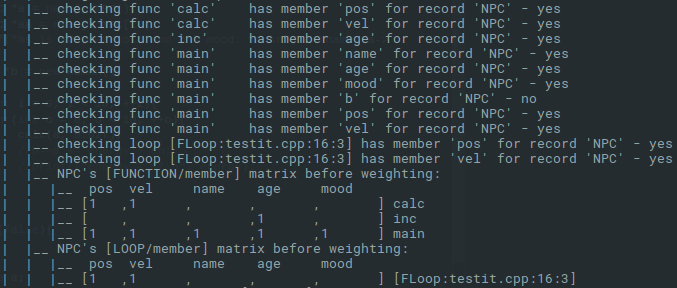
\includegraphics[width=.7\linewidth, height=0.3\linewidth]{PICs/npc_crosscheck_matrix}
	\caption{Excerpt of coops output on exemplary NPC and some arbitrary functions/loops}\label{npc_crosscheck_matrix}
\end{figure}
Ultimately our evaluation faces a problem, that scales with our implementation details. Similarly to how we evaluated cache-line utilization in \refsec{soa} for each function we could determine (estimate) its behavior for a certain Hot/Cold split in a brute force kind of way. So we can make statements about which split would be the best.\\
Through a function/member matrix we can determine cache utilization for each function individually. The number associated with a member expression can be interpreted as 'how much punishment would it mean to externalize me for this function'. For a simple case like \reffig{npc_crosscheck_matrix} we could easily determine, that the function \textit{calc} would like to have the \textit{name, age, mood} field subset externalized. But externalizing either \textit{pos} or \textit{vel} would mean loading the respective cold struct instance as many times, as it's associated value. The \textit{punishment} specifically would depend on how big the cold struct instance is, which also varies depending on whether or not each other field is hot or cold.\\
More formally there are $\sum_{k=0}^{n} \frac{n!}{k!(n-k)!}$ different combinations of how a record can be split, where $n$ is the number of fields in the record and $k$ is the number of fields to hive off. As an example we could imagine a record with 10 fields. Conclusively there are 1023 different combinations of possible splits. Checking each function lets say 50 would result in $> 50.000$ computations. Since we specifically regard the loops as well this number will become even higher - per record - and eventually with actual big code bases shoot through the roof.\\
So instead of cross checking each split scenario with each function/loop we would like to consolidate each fields 'importance' or it's 'weight' in a centralized spot, that will be checked against $n-1$ other fields instead.

\subsection{Metric for evaluation of field usages}\label{metrics}
We described fields to have relations to loops/functions. Expressing these relations numerically might get us into regarding existing metrics, hoping they provide information we can process. The values assigned to a relation could be based on a lot of things, so at this point we should contemplate on what would be the most useful piece of information. Even though we will see, that the chosen metrics do not suffice our needs perfectly, they have aspects and methodology we can utilize for our purpose.
\subsubsection{Cohesion metrics}
An automated Hot/Cold Split will eventually externalize a subset of fields into another record. We do so by finding the hot data and conversely the cold data \refsecp{hot_cold_splitting}. When thinking about why the cold data was put together with the hot data in the first place we remember, that it might be due to our unfortunate abstraction \refsecp{oop_bad_abstraction}. Talking about splitting records on account of their fields' relations sounds like what \textit{cohesion metrics} try to solve.\\
Cohesion in a module describes to what extend, that module serves a single logical task \mcp{ingeno_cohesion}{172}. Its purpose is to indicate on how well a software architecture is defined. Modules with good cohesion have proven to be reusable and easy to maintain, whereas low cohesion indicates, that changes in the code will affect other parts of the code resulting in increased effort in development as well as in testing \mcp{ingeno_cohesion}{172}.\\
There are several types of cohesion, that are used to classify a module, like \textit{Coincidental Cohesion}, where elements are grouped with no logic concept for example in a utility or helper collection. This is considered to be low cohesion and should be avoided.\\
\textit{Logical Cohesion} describes what we have found to be bad abstraction patterns coming with OOP. We group logically related elements, because they share a context. Consequently we will collect lots of fields, that belong to different domains. Cohesion metrics also recommend to avoid this kind of design.\\
\textit{Temporal/Procedural Cohesion} both describe a grouping of fields, because they are processed at the same time/in a certain order. So basically when they share temporal locality. Even though we discussed earlier \refsecp{cpucu} that trying to design around principles of locality is one of our main goals in DoD, thinking in an OOP way this is rather bad, because it might promote monolithic class- and method definitions. Again cohesion metrics want our record definitions to follow a single task. This level of cohesion is considered to be acceptable but not ideal \mcp{ingeno_cohesion}{174}. But DoD doesn't argue here actually. Temporal/Procedural cohesion think in a bigger scale than what we meant earlier with temporal locality. For example grouping independent elements because they all are related to system startup/cleanup even though they don't interact.\\
This is another example of where we find a big gap between OOP and DoD at first glance but they actually conform with each other for the most part, only differing in motivation.\\
Working our way up to the notion of an \textit{ideally} cohesive model, we pass a few other levels until we reach \textit{Functional Cohesion}. This level describes a module to group elements sharing a domain. The module will therefore serve a single purpose and changes to it won't affect code of other domains. Note that OOP very well allows for good abstraction, but again the inherent problem we face is that our intuitive abstractions don't accommodate neither software design nor our hardware. More importantly this definition of 'desirable cohesion' fits our needs to implement a Hot/Cold split, so cohesion metrics might bear the right tools, to accommodate us.\\\\
There are a bunch of metrics like \textit{LCC} (Loose Class Cohesion)  and  \textit{TCC}  (Tight  Class  Cohesion)\mcp{tcclcc}{3} or the famous \textit{LCOM} (Lack of Cohesion in Methods) \mcp{cohesion}{25}. Since cohesion metrics operate on object oriented code, they usually work with methods, as groups of field subsets. For example the LCOM defines a module's cohesiveness to be the "\textit{number of pairs of methods operating on disjoint sets of instance variables, reduced by the number of method pairs acting on at least one shared instance variable}"\mcp{lcom}{8}.\\
While cohesion metrics have a striking similarity in their procedure (splitting records according to their field usages), unfortunately they do differ in their intention and result. As for our Hot/Cold split, we intend to be a performance optimization and are ready to group any fields, that share spatial/temporal locality. Ultimately our Hot/Cold Split will usually automatically divide a record into domain specific sub sets, its focus however is to minimize a record's stride for cache utilization. This means we could easily end up externalizing a domain related field for the sake of faster computation.\\\\
But all is not lost, because cohesion metrics provide us with proven methodology to identify and evaluate relations in a module (record) in numbers we can compare. We also learned, that to better fit our purpose, a target metric should regard our code's performance and/or size (memory stride). 

\subsubsection{Asymptotic Notations}
An asymptotic notation or more famously O-notations describe an algorithm's complexity \mcp{onotation}{44}. It is not a measurement tool to actually evaluate the performance or memory size an algorithm uses since these depend on hardware/architecture/compilers. It describes how an algorithm scales depending on the problem size and defines upper-/lower borders for it's (asymptotic) growth depending on which notation is used. Hence the name because it deals with the \textit{order} of an algorithm.
There is for example the $\Theta$-notation that expresses asymptotic upper- and lower bounds for a given procedure.
Specifically the Big O-notation (or Landau's symbol) describes the worst-case for a procedure (asymptotic upper bound). Dealing with bounds makes sense because depending on the input (problem size), performance as well as needed memory space might vary drastically. Using the O-notation we can get estimations about a functions running time only by looking at its overall structure \mcp{onotation}{47}\\
An actual static performance analysis of code would break down the instructions to those we can find in the hardware's instruction set (depends also on the compiler), to get a grasp of how many cycles they need and ultimately how a cycle translates to (probably) nanoseconds.\\
The O-notation in its essence will also look at the instructions a procedure makes, when looking at the code. However it builds terms by evaluating control flow statements and eventually will omit constants and all but the highest order term. Expressed as a polynomial $g(n) = 5n^2+3n$ would translate to $g(n) = O(n^2)$. Since $g(n)$ is of order $n^2$ the equals notation is not perfectly correct but commonly used. Leaving out constants and low order terms is due to their insignificance considering large $n$. After all it describes asymptotic behavior.\\
In the best case a procedure is of order $O(1)$, which means no matter how big the problem becomes it won't affect our performance further. This is the case for each procedure, that operates on a fixed amount of parameters (for example typical getters/setters). While even a setter can consist of several instructions, lets say for example 3, it would translate to $3\cdot O(1)$. After omitting the constant $3$ we are left with $O(1)$. It is referred to as \textit{constant} growth.\\
Loops oftentimes iterate over dynamic ranges, so when a loop is operating instructions $n$ times it is denoted as $O(n)$ or has \textit{linear} growth.\\
Nested loops are often denoted as $O(N\cdot M)$, where N and M represent the iterations for the outer- and inner loop. In cases where N and M are equal we refer to it as \textit{exponential} growth or $O(n^2)$.\\\\
For our use case classifying our functions like this could be useful. After identifying the relevant functions (those that use our records' fields), we could evaluate them by determining their order. We could see which functions are the 'slowest' and thus reduce memory stride on the records they utilize. This could work by simply defining each field, that is used in those functions as hot. Functions that are known, to be slow, could now operate on hot data exclusively.\\\\
Unfortunately this bears some problems. A high ordered function might interact with our records very briefly (or not at all), yet would be considered a criteria for deciding which fields are hot/cold. This alone illustrates why we can't blindly apply asymptotic bounds as a criteria. We have to adapt it to our motivation, by only considering or prioritizing instructions, that are (or imply) field usages, yet again only considering our fields might falsify a denotation of the function.\\
There often won't be the one slow function, the \textit{single point of bottleneck}. Identifying a functions members as hot, in order to speed up that function might work, but might just as well worsen each other remaining function. Whether or not a field is to be considered hot has to be determined individually with their groupings (uses in functions) as a relevant indicator rather than a decisive factor.\\
Omitting constants and low order terms might provide fair estimations for large $n$, but not every program operates on huge amounts of data. Of course software, that doesn't depend on its data layout very much probably won't significantly benefit from a Hot/Cold split, but lower order parts of a procedure might affect the performance enough for them to deserve to have a say. Also they might be useful deciding factors in close calls.\\\\
Again all is not lost. Asymptotic notations provide us with useful policies to determine a procedure's complexity. We can adapt the way it reflects on constant; linear; quadratic etc. growth, to derive an evaluation for the fields it uses. 
\newline
\subsubsection{Quantitative cohesion alternation}
\begin{wrapfigure}[21]{r}{0.4\textwidth}
%\vspace{-45pt}
\begin{lstlisting}[language=C++, name={Exemplary pseudo-ish code}, label={exem_code}]
void inc(Foo &foo){
	foo.age += 1;
}
...
void p2(Foo &foo){
	foo.bar *= foo.bar;
}
...
bool gt(Foo &foo1,
  Foo &foo2)
{
	return
		foo1.bar > foo2.bar;
}
...
for(Foo *foo : all_foos){
	inc(*foo);
}
...
for(int i = 0; i < N; ++i)
for(int o = i+1; o < N; ++o)
collision(foos[i], foos[o]);
\end{lstlisting}
\end{wrapfigure}
Now that we have found procedures, solving our problem partially we might be able to derive a fitting methodology. A first approach could be to try to evaluate field usages (non method member expressions) similarly like we would evaluate statements for an asymptotic notation. As a simple start we could count the amount of member expressions per function. Considering something like \refcode{exem_code} the \textit{inc} function in line 1 could be evaluated easily. We have one member expression \textit{foo.age}.\\
When looking at the \textit{p2} function in line five we notice that our scheme would now rate p2's relation to the field \textit{Foo::bar} as a 2, since it occurs two times. Hence the field \textit{Foo::bar} would be considered \textit{hotter} than the field \textit{Foo::age}.\\
But do we want this behavior? Cohesion metrics like LCOM don't count all field usages of a specific field for one method, but group them in sets for each method instead. This way it is not about which field is the most prominent one, but which fields share related context. Even though it is a true observation, that bar is used more often than age (at this point), considering the cache there is only one \textit{Foo::bar} to work with. There is however an important difference to cohesion metrics we need to consider. Even though we are interested in domain relations (field groups) our cache utilization highly depends on which fields are loaded most frequently. The \textit{gt} function (line 9) on the other hand uses two distinct \textit{Foo::bar}s (assuming strict aliasing). \textit{gt} will actually be responsible for loading two addressable units into the cache. A reduced stride between relevant data could be more efficient here (this situation should be prioritized over \textit{inc/p2}). Depending on how big an actual Foo instance is and how many distinct \textit{Foo::bar} fields are accessed in one function counting \textit{distinct field usages} might be a more helpful evaluation of a relation. This is a cache conscious compromise between detecting domain relations, but prioritizing load frequency.\\\\
The access patterns that start to make things spicy for the cache however are usually loops.
\begin{quote}
	\textit{Loops have good temporal and spatial locality [...] the greater the number of loop iterations, the better the locality.} \mcp{bryant}{589}.
\end{quote}
When looking at line 16 to 18 of \refcode{exem_code} the for-loop iterating an arbitrary number of Foos might outclass any simple function, even if that function is using dozens of distinct fields - hard coded. There is only one field usage to see, yet it could constitute numerous instances. That is why asymptotic notations evaluate loops like these with \textit{linear growth}.\\
Even though a loop's amount of repetitions can sometimes be evaluated at compile time, in OOP where objects tend to be created on the heap and their containers are extended dynamically there is no real telling just how much distinct instances of field usages there will be. So we know, that loops might be game-changers for our evaluation, but as a matter of fact we can't ever predict a perfect number of recurrence. So either we rely on helper indices/iterators, make a few test runs to log and memorize their peaks, or we try to find a reasonable estimation. Like the O-notation we might remember loops and associate them with an arbitrary factor \textit{n} for now, but for an actual comparison of the fields, later we will need to decide how to rate them.\\
This estimated value we are going to associate with a field usage inside a loop could be based on experience but the best we are ever going to get out of experience is "\textit{entirely depends on the use case}". A better way of evaluating a loops impact is in a way for it to not break our scale immediately, but allowing it to do so. Whats meant by that is the fact, that associating a field usage inside a loop with a number that is vastly higher than that of a function, will render our functions meaningless quickly. However the moment we start nesting loops inside each other (allowing for \textit{quadratic/polynomial growth}), calling single functions impact-less might actually be true. Besides opposed to asymptotic notations we won't rigorously drop lower order terms, we will just make sure, that an expression is allowed to be much more significant.\\
Facing reality nested loops hold the greatest potential for bad cache utilization, since they can repeatedly load irrelevant data on several iterations. Our scale will definitely end up starting at a low level listing single function accesses on data then at some point rapidly going up where nested loops reside together. Line 20 to 22 in \refcode{exem_code} will quickly outperform other control flow statements and while a nested for loop like this is no rarity the \textit{loop depth} of a statement, can be arbitrarily high/deep, depending on the situation.\\
In order to actually account for an expression's loop depth we will need measures that will be discussed in \refsec{project_scope_transformations}. For now we imagine having instant access on them.\\\\
In terms of implementation, COOP remembers each function and each loop individually, as well as the member expressions they contain respectively. After data aggregation with the matchers and their callback routines we can create function/member and loop/member matrices like in \reffig{npc_crosscheck_matrix} for each record.\\
Just like cohesion metrics we can use field subsets used in functions to declare contextual relation, assuming temporal locality through AST node familiarity. Meaning each row (function) embodies a relation between the fields it uses \reffigp{npc_crosscheck_matrix_relations}. Each value inside such matrix stands for the computational \textit{weight} of that field for the function. A column represents a field's distribution among the functions. Totalizing a column determines the field's overall weight that will eventually be used to compare it to the others.
\begin{figure}[!htbp]
	\centering
	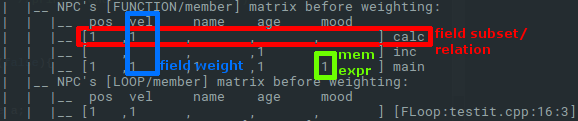
\includegraphics[width=0.7\textwidth, height=0.2\textwidth]{PICs/npc_crosscheck_matrix_relations}
	\caption{Relations depicted in function/member matrices}\label{npc_crosscheck_matrix_relations}
\end{figure}
Fields' relations to each other need to be valued, too. After all their correlation will work best, if they end up as hot data together. The aim is for their temporal locality to result in improved spatial locality. Each group of field usages (function) needs to somehow weight its collective field impact, to heighten their chance to stay together as hot data. We prioritize small groups, since externalizing more fields (with low usage frequency) will result in less stride. Functions will therefore compete against each other, by adding to their field weights the overall number of fields minus the amount of fields they utilize. This scales with the number of fields a record has. As mentioned before instead of brute forcing our way through each possible split combination we now encode each field subset relation numerically so eventually it will influence a field's overall weight. It is important to form a decision over an overall weight because unlike an optimization for a specific algorithm, changing the programs data layout has the potential to affect ALL of its functions.

\subsection{Field weight heuristics}\label{field_weight_heuristics}
When we are able to define a field's overall weight on a program, whats left to do is finding a delimiter, that actually divides the field set in two subsets, depending on those weights. This again is not a trivial operation and first of all we need to define what we intend to separate.\\
As can be seen in the Figures \ref{avg_delimiter} to \ref{avg_delimiter_bad_5} we will face numerous different situations that result of arbitrary access patterns. While sometimes it is easy to rule out certain fields for others it is not. A generic set of rules to handle this needs to be able to process special cases while not losing credibility for common ones. It can do so by scaling with the problem.
\subsubsection{Scaling delimiters}
Scaling delimiters will adjust automatically as the problem changes. In a lot of cases a very easy heuristic will work comparably well. For example a (we will call it) \textit{max/2} where we will just take the maximum field weight and divide it by two. Everything above the \textit{max/2} will be hot and vice versa. Given our 'scope' is the maximum field weight this will yield very good results for a lot of cases, however the more significant the spikes are, the worse will be the affects on the resulting data layout. While the \textit{max/2} regards quality it dismisses quantitative scaling.\\\\
A surprisingly easy yet effective candidate is the average, because it scales up when certain fields tend to be a lot more important than others and naturally divides our values according to their relative weight \reffigp{avg_delimiter} unlike for example their median value.
\begin{figure}[ht]
	\begin{minipage}[b]{0.5\linewidth}
		\centering
		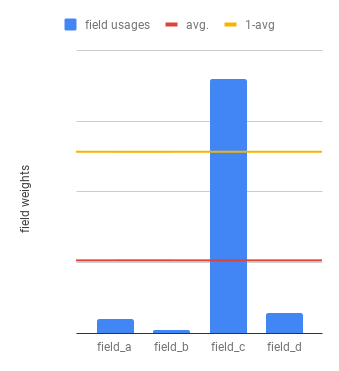
\includegraphics[width=\textwidth,height=.7\textwidth]{PICs/avg_as_delimiter_1}
		\caption{Good avg scaling.}
		\label{avg_delimiter}
	\end{minipage}
	\hspace{0.5cm}
	\begin{minipage}[b]{0.5\linewidth}
		\centering
		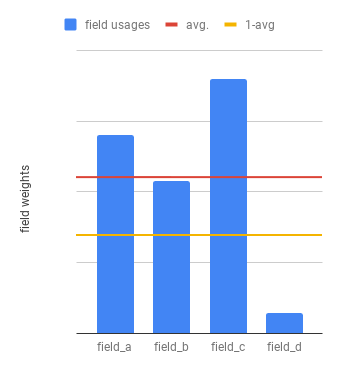
\includegraphics[width=\textwidth,height=.7\textwidth]{PICs/avg_as_delimiter_2}
		\caption{Difficult evaluation for avg scaling.}
		\label{avg_delimiter_bad}
	\end{minipage}
	\hspace{0.5cm}
	\begin{minipage}[b]{0.5\linewidth}
		\centering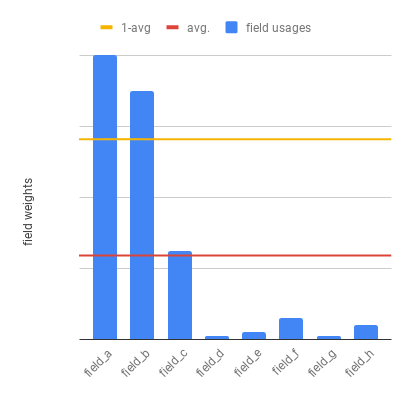
\includegraphics[width=\textwidth,height=0.7\textwidth]{PICs/avg_as_delimiter_3}
		\caption{Bad avg scaling with more fields.}
		\label{avg_delimiter_bad_2}
	\end{minipage}
	\hspace{0.5cm}
	\begin{minipage}[b]{0.5\linewidth}
		\centering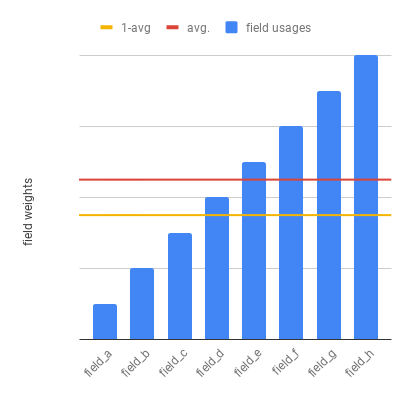
\includegraphics[width=\textwidth,height=0.7\textwidth]{PICs/avg_as_delimiter_4}
		\caption{Problem of even distribution.}
		\label{avg_delimiter_bad_3}
	\end{minipage}
\end{figure}
Unfortunately \reffig{avg_delimiter_bad} shows, why sometimes a simple average determination might not be the best fit. If \textit{field\_a} or \textit{field\_c} were slightly less important, \textit{field\_b} would probably be considered hot, yet this way, even though it's rating is far from \textit{impactless} it is considered to be cold.\\
On the other hand \reffig{avg_delimiter_bad_2} shows why an average will also not scale well with the amount of fields in a record. The average narrows as the divisor grows, so on a record with a hand full of members an average might end up introducing fields to the hot subset that barely pass the average weight.\\\\
This leads to an interesting dilemma. Where to draw the line between hot and cold fields? Should there be constant \textit{magic numbers} defining the threshold of a hot field? Since different access patterns can produce arbitrary field weightings there is no good way of predicting a constant, that suffices our intention. But how can relative proportions work when they introduce false-positives? And can we get rid of them? \reffig{avg_delimiter_bad_3} illustrates a difficult case that will in practice rarely occur but embodies our problem perfectly. An even distribution of field weights allows for no logical grouping of significance, at least in terms of 'drawing the line'.
\begin{figure}[ht]
	\begin{minipage}[b]{0.5\linewidth}
		\centering
		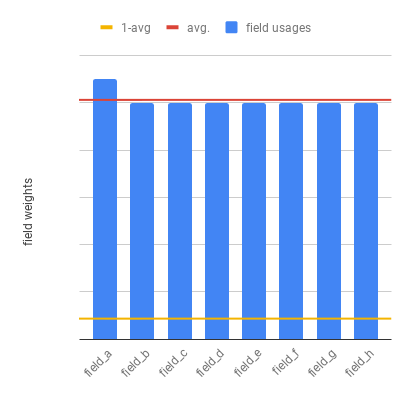
\includegraphics[width=\textwidth,height=.7\textwidth]{PICs/avg_as_delimiter_5}
		\caption{Bad avg homogeneous field weights.}
		\label{avg_delimiter_bad_4}
	\end{minipage}
	\hspace{0.5cm}
	\begin{minipage}[b]{0.5\linewidth}
		\centering
		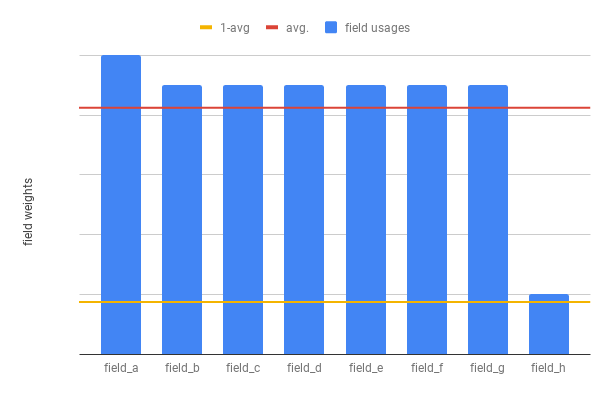
\includegraphics[width=\textwidth,height=.7\textwidth]{PICs/avg_as_delimiter_6}
		\caption{\textit{1-avg} prone to false positives as well.}
		\label{avg_delimiter_bad_5}
	\end{minipage}
\end{figure}
The average as a heuristic fails us in many situations. We referred to it because it provides a quick approximation of a good delimiter. The factors however that determine its scaling are contrary to the paradigms we follow. Number-of-fields as a divisor means decreasing averages with increasing amount of fields. This means the more fields our records have (consequently the more lack of cohesion), the higher the collective chance to be considered hot. Also the average behaves poorly towards well designed records. Consider \reffig{avg_delimiter_bad_4} where \textit{field\_a}'s weight is just slightly higher than the others'. It will deem all fields but \textit{field\_a} cold and probably ruin the data layout.\\\\
The above diagrams propose another heuristic that we will call the \textit{1-avg}, represented by the yellow lines. It introduces the reciprocal counterpart for the averages bad scalings. By taking the greatest field height minus the average, our tolerance for fields grows linearly as the average rises while regarding the overall scope of our field weights. In other words: The more quality we find in a record (the more the average trends towards the maximum field weight) the more fields we allow to be hot.\\
As can be seen in the above figures, this heuristic behaves much better for records that show great differences in their field weights. Of course it is very much possible for it to behave poorly in specific situations as well, again coming from spikes. \reffig{avg_delimiter_bad_5} shows, that the reciprocal average quickly becomes too tolerant. We have seen, that \textit{1-avg} is able to correct some mistakes the average makes but it introduces unwanted behavior on its own.\\

\subsubsection{Combined scaling delimiters}
An interesting take is on how to combine certain scaling delimiters. Depending on the case different heuristics will result in drastic deterioration of the data layout. We could try to get rid of errors by cherry-picking the strengths different heuristics provide.\\
One possibility could be to adapt the \textit{max/2} heuristic. We can determine both the \textit{avg} and the \textit{1-avg} delimiters, take the greater one and divide it by 2 (we will call it \textit{top/2}). The upper delimiter will always separate the most significant fields for us. As the \textit{max/2} easily gave us a quick way of defining a tolerance towards lower significant fields, it did not in any way regard the fields' quantity as a defining factor. By possibly considering the \textit{1-avg} (when it is greater) we adapt it given the right situation. This already yields improved results, is however still prone to special cases \reffigp{top_2}. This is because we don't consider the possibility of the cold remnant to be relevant in its entirety.
\begin{figure}[!ht]
	\begin{minipage}[b]{0.5\linewidth}
		\centering
		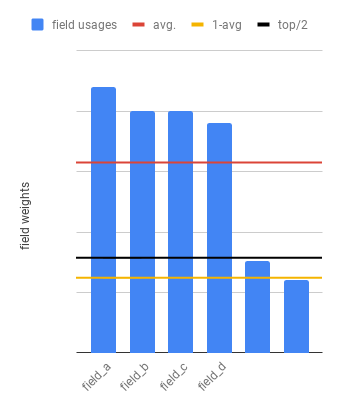
\includegraphics[width=\textwidth,height=.8\textwidth]{PICs/top_2}	
	\end{minipage}
	\hspace{0.5cm}
	\begin{minipage}[b]{0.5\linewidth}
		\centering
		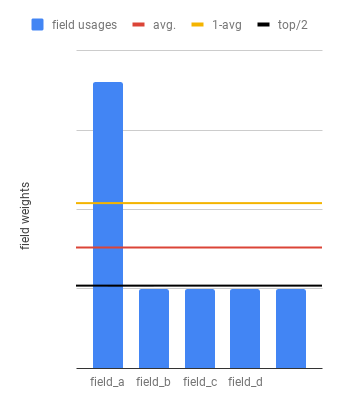
\includegraphics[width=\textwidth,height=.8\textwidth]{PICs/top_2_bad}
	\end{minipage}
	\caption{Improved \textit{top/2} heuristic as it is able to rule out \textit{1-avg} errors but still not well.}\label{top_2}
\end{figure}
The problem with scaling delimiters is, that no matter how much we narrow down the error by applying a certain heuristic, in another distribution the same approach might behave badly in terms of handling another error source. We need to evaluate subsets of fields ordered by significance to reliably rule them out or keep them collectively.\\\\
Regarding both the \textit{avg} and the \textit{1-avg} is interesting because combined they are able to categorize the field weights to a certain extend. As mentioned before, there are two major scaling factors the fields' weights and their number. As the \textit{1-avg} is the reciprocal of the \textit{avg} we can derive information about a programs access patterns by looking whether \textit{avg} or \textit{1-avg} is greater than the other.\\
When the \textit{avg} is greater, the fields' weights is proportionally more significant than the record's number of fields. When the \textit{1-avg} is greater on the other hand, it means that proportionally there are more insignificant fields, than the subgroup of 'important/hot' fields. Well designed records will demonstrate $avg\approx f_{max}$. Anyhow we can interpret those two delimiters as an order of significance. They divide our scope into three spaces. One above the greater delimiter, one below the smaller delimiter and whatever is in between them \reffigp{delimiter_tiers}. Fields in the upper space are certainly to be considered hot. Fields below the lower line are in a less significant order. Whatever is in between is what we can not categorize immediately. 
\begin{figure}[!ht]
	\begin{minipage}[b]{0.5\linewidth}
		\centering
		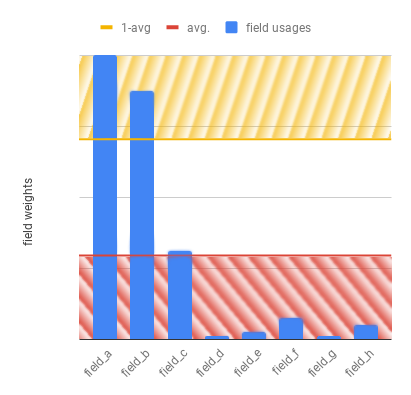
\includegraphics[width=\textwidth,height=.7\textwidth]{PICs/delimiter_tiers}	
	\end{minipage}
	\hspace{0.5cm}
	\begin{minipage}[b]{0.5\linewidth}
		\centering
		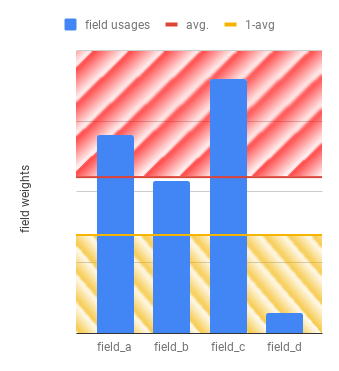
\includegraphics[width=\textwidth,height=.7\textwidth]{PICs/delimiter_tiers_2}
	\end{minipage}
	\caption{Field weight categorization by combined scaling delimiters. Top hatched space is of high significance.}\label{delimiter_tiers}
\end{figure}
The idea is to now recursively apply the ordering between the \textit{avg} and the \textit{1-avg} delimiters as long as we have fields, that we can neither classify as high- nor little significance. This approach will work fine with data sets, that exhibit high significance varieties. On uniformly distributed field weights it will tend to include the whole field set for the hot data, yet since we encoded logical relations in the field weight a distribution like in Figure \ref{avg_delimiter_bad_3} bespeaks of defective access patterns rather than only bad data layout.\\
Regarding order of significance is a good approach to a generic solution, yet our recursive approach is not optimal since it is based on scaling delimiters, that are unaware of a field-group's collective impact. Also trying to break down a record's significance order into two (hot \& cold) subsets immediately mitigates precision.

\subsubsection{Order of significance / Significance groups}\label{sig_groups}
The problem is that until now we tried to divide a record in two subsets. This is actually what we want, but the truth is there can be an arbitrary amount of related subsets in the record's data fields and the more significance groups we have and the greater the difference in significance, the blurrier the delimiter becomes. Delimiters based on either quantitative or qualitative scaling introduce an error of a size we can hardly reason about when compared to the entirety of field weights \reffigp{delimiter_bad}. Percental tolerance factors will also always just move the error resulting in better behavior in some situations and worse in others.\\
Also one of the worst situations for us is to accidentally separate fields, that are logically related. With scaling delimiters it can easily happen, that two fields, that share an order of significance (due to our metric) are separated because the delimiter ever so slightly includes one of them but excludes the other. Whenever we split fields that are codependent we ensure worsened cache utilization, because the functions that use the hot field will most likely also use the cold field and will now have the additional overhead of the indirection to the cold struct instance. Our Recursive approach tried to solve this issue and will succeed in simple cases, yet ultimately it depends on the blurry scaling delimiters.\\\\
Scaling delimiters try to evaluate field weights individually, yet their sub-/optimal utilization strongly depends on their significance group. Determining whether or not a field should be considered hot should depend on the benefit/punishment of it's extraction. Externalizing a field always means that the remaining hot fields load less unnecessary stride into a cache-line, yet it also means whenever the extracted field is used unrelated cold data might be loaded as well.\\
Cache-lines have concrete sizes (e.g. 64 Byte) so at this point we might be tempted to just multiply a field's size in byte to it's weight. This way we could see the fields impact on the cache capacity and evaluate whether or not determining a certain field as cold would imply great punishment. But this way the least frequently used field could suddenly be considered hot if it is just big enough. We may not confuse capacity with usage frequency, which is the actual criteria of a Hot/Cold Split \refsec{hot_cold_splitting}. So it is actually enough to compare our field weights as a criteria for benefit and punishment. However in order to determine a significance group's impact on our program we are definitely interested in comparing its size to the cache-line size in order to deduce possible stride (which we want to reduce after all).\\\\
But how can we determine significance groups? COOPs approach is to sort the fields according to their weights in a descending order and measure their weight differences. Normalized on the scope ($f_{max}$) we can compare them to the average deviation. Each value above the average will denote a new less significant group that spans until the next group is identified \reffigp{sig_order}.
\begin{figure}[ht]
	\begin{minipage}[b]{0.5\linewidth}
		\centering
		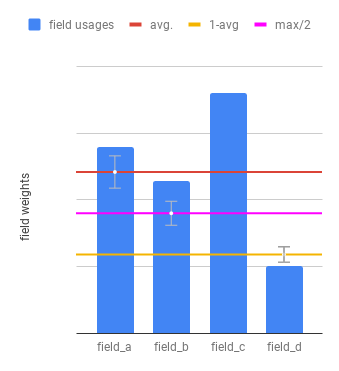
\includegraphics[width=0.8\textwidth,height=.7\textwidth]{PICs/delimiter_bad}
		\caption{Scaling delimiters' errors can hardly be reasoned about and provide equally much punishment as benefit depending on the distribution.}
		\label{delimiter_bad}
	\end{minipage}
	\hspace{0.5cm}
	\begin{minipage}[b]{0.5\linewidth}
		\centering
		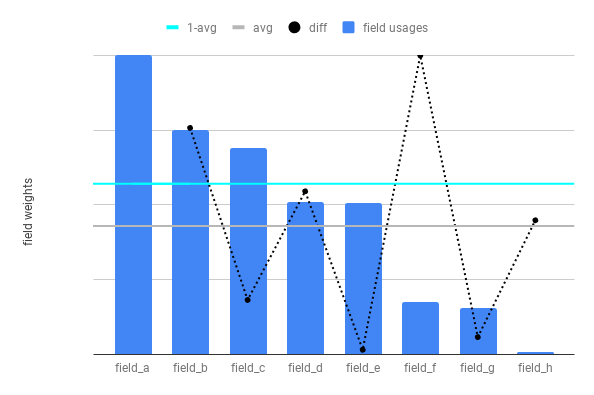
\includegraphics[width=\textwidth,height=.7\textwidth]{PICs/sig_order}
		\caption{Determination of significance groups with field weight deltas. Normalized differences are projected on the field weights' scale for visualization.}
		\label{sig_order}
	\end{minipage}
\end{figure}
The important thing is for the fields to be evaluated in terms of groups rather than individually. How to evaluate a group though? First we need to determine the group's benefit/punishment in case of a split. Each significance group $g_i$ has a type size $s_i$ which is the summarized type sizes of it's fields, as well as a $max_i$ which is it's highest field weight. With the cache-line size $CLS$, the general cold struct indirection overhead $H$ and with $n$ as the amount of significance groups, when a group $g_i$ is extracted, it implies the following:\\
Extracting $g_i$ means $s_i$ less stride for the remaining hot data. We already ordered the fields' weights in a descending order, so now we can compare their type sizes with the additional space and as soon, as one or more of the hot fields fit in the additional space (minus $H$) we will effectively have reduced the number of cache-lines to fit 1 hot data instance by the factor $\frac{s_i}{CLS}$ (without splitting an addressable unit over two cache-lines). So the benefit will express through the re-utilization of the hot fields which is capped to the highest field weight of the hot fields ($F_{max}$ or $max_0$). We can value it by multiplying the $F_{max}$ with the determined benefit. This practically tells us how many cache-lines we will spare our important procedures.\\
But we can make our estimation a little better by interpreting each significance group as a representation for those procedures (loops/functions), that have contributed to it. So instead of capping our 'savings' estimation on the most significant value ($F_{max}$) we will take each significance groups maximal field weight, as this value represents the groups estimated loads. So our savings $s(g)$ are:
\begin{align}
	s(g_i) = \sum_{k=0}^{i-1}max_k\cdot\frac{-H+\sum_{k=i}^{n}s_k}{CLS}
\end{align}
At this point our procedure will cut off everything until the last group of highest significance, because we have not yet determined the 'costs' of externalizing a significance group as a counter weight. As the stride is reduced for the hot subset it is increased in the cold subset. The payoff for a hot set is the additional indirection over the pointer to the cold struct instance. When applied correctly this is however comparably little as we plan to externalize greater means.\\
The cold data will always be accessed by going through the hot data (the pointer to the cold data is in the hot data). So whenever we are accessing cold data we automatically waste one cache-line per cold struct instance that is used to load and dereference the pointer to it. In terms of cache utilization this is really bad (not only in terms of capacity, but also because of possible thrashing since the hot and cold data lie at physically different locations \refsecp{cpucu}). Its only worth because we do it with data, that is accessed so rarely (relatively), that this cost is lower than the benefit we get by splitting it from the hot data. However, besides the additionally wasted cache-lines used solely for finding the actual data, we will increase the cold data's stride by $s_i$ Byte, resulting in an estimated iteration overhead $o(g)$ of
\begin{align}
	o(g_i) = \sum_{k=i}^{n}max_k\cdot(1+\frac{\sum_{k=i}^{n}s_k}{CLS})
\end{align}
cache-lines for processing the cold data in its entirety. Ultimately for each $g_i$ we say that a split is worth $w(g)$ when:
\begin{align}
	w(g_i) = s(g_i) > o(g_i)
\end{align}
Then we want to externalize it because the estimated benefit is greater than the estimated cost.\\\\
Unfortunately this will only work for tightly packed arrays of data, since we assume, that reduced stride immediately results in improved cache utilization. If we implemented an automatic SOA transformation this would be the way to go \refsecp{soa}. Due to alignment issues (more on that in TODO REF SEC) COOP will allocate the hot and cold data in a way that is not exactly packed, but will consider alignments, so to a certain extend a reduced stride will have virtually no effect other than the additional indirection to the cold data - invalidating our progress so far.\\
To be more specific COOP will regard the target systems L1 D (configurable depending on optimization preferences) cache-line size and will try to pack as many elements into a line, yet align each entity group to the cache-lines, to prevent unnecessarily much entity splits over too many cache-lines  (we briefly discussed this in \refsec{aosoa}). This means, that when our hot subset size is smaller than the target cache-line, reducing the stride will have effect, as soon as it frees enough space for the cache-line to encompass another instance \reffigp{opt_p_1}.\\
On the other hand, if the hot subset size is greater than the cache-line, reduced stride will have effect, as soon as it results in reducing the number of cache-lines necessary to encompass an instance \reffigp{opt_p_2}. So actually since we will introduce padding due to our alignment we might even want to consider keeping poorly ranked fields, as long as they only replace space, that otherwise would be used for padding.
\begin{figure}[ht]
	\begin{minipage}[b]{0.5\linewidth}
		\centering
		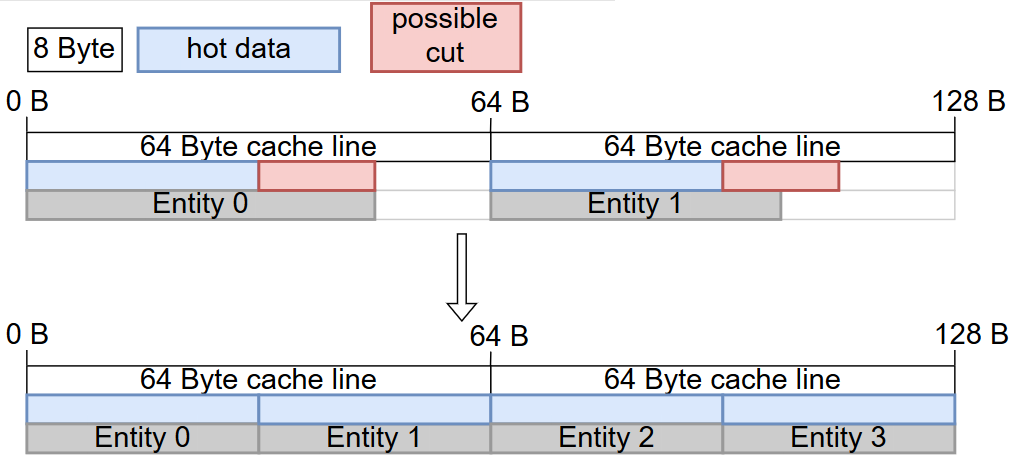
\includegraphics[width=\textwidth,height=.6\textwidth]{PICs/opt_possibility_1}
		\caption{Aligned entities will be packed inside cache-lines. Reduced stride will be effective, as soon as it increases the amount of entities inside a cache-line.}
		\label{opt_p_1}
	\end{minipage}
	\hspace{0.5cm}
	\begin{minipage}[b]{0.5\linewidth}
		\centering
		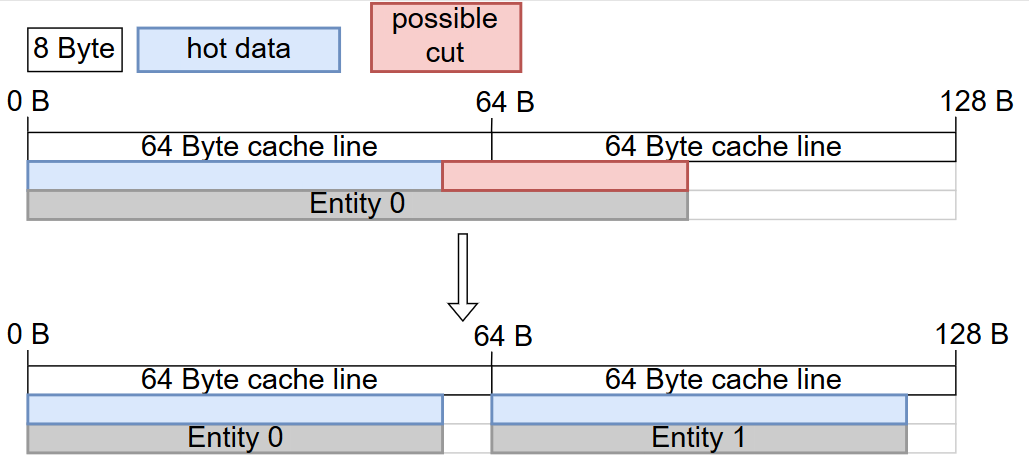
\includegraphics[width=\textwidth,height=.6\textwidth]{PICs/opt_possibility_2}
		\caption{Reduced stride will be effective as soon as it reduces the number of cache-lines needed to encompass an entity. Entities are split upon minimum amount of lines.}
		\label{opt_p_2}
	\end{minipage}
\end{figure}
Again this needs proper evaluation, since at this point our procedure will blindly cut out fields because it can't reason about the splits impact to it's full extent. We again need to include our field weights into the equation, to be able to evaluate whether or not a split will result in more benefit, than punishment.
More formally for a significance group $g_i$ our heuristic $W(g)$ will consider a split beneficial when:
\begin{equation*}
W(g_i) =
\begin{cases}
\scalemath{1.2}{\myceil{\frac{CLS}{\sum_{k=0}^{i-1}s_k}}} > \scalemath{1.2}{\myceil{\frac{CLS}{\sum_{k=0}^{i}s_k}}} \land w(g_i) & \text{for}\sum_{k=0}^{n}s_k < CLS\\\\
\scalemath{1.2}{\myceil{\frac{\sum_{k=0}^{i-1}s_k}{CLS}}} < \scalemath{1.2}{\myceil{\frac{\sum_{k=0}^{i}s_k}{CLS}}} \land w(g_i) & \text{for}\sum_{k=0}^{n}s_k > CLS
\end{cases}
\end{equation*}
It is worth to note here, that this consideration of the groups type sizes is another kind of scaling that we haven't had considered before. This heuristic will yield different results depending on the actual type sizes and will therefore be more precise in its evaluation. Scaling delimiters solely relying on comparing the field weights will tend to split over aggressively, because they don't consider that the benefit of a split depends also on how the resulted record's will interact with a specific target cache. In fact to actually accomplish an improvement a cut will now need to extend a certain threshold. So in many cases COOP will now rather do nothing, than trying to force a split, that will actually worsen the cache utilization.\\\\
\begin{figure}[tbp]
	\centering
	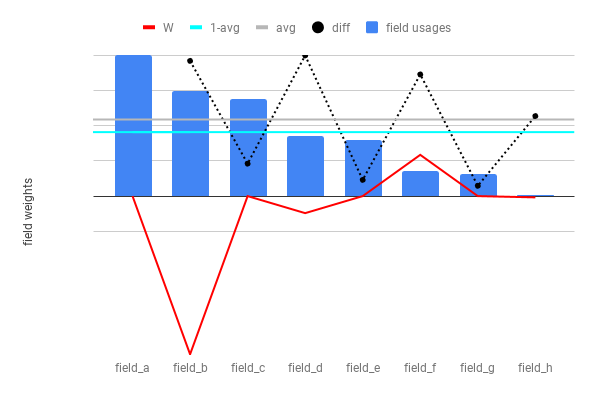
\includegraphics[width=0.8\textwidth,height=0.5\textwidth]{PICs/sig_order_final}
	\caption{Exemplary field weights evaluated by our heuristic with the result, that its worth to make the split hot:[\textit{field\_a}, ...\textit{field\_e}], cold:[\textit{field\_d}, ...\textit{field\_h}].}
	\label{sig_order_final}
\end{figure}
Unfortunately this heuristic might be problematic, as soon as we deal with significant spikes. Imagine a field, that outweighs the others. Since we only consider significance groups as split candidates (opposed to fields individually) we will now compare $n-1$ fields to be split. This might actually make sense, because the highly rated single field might provide well enough cache utilization to outweigh the externalization of the rest, however we will strip ourselves from optimization potential as soon, as deviation significance leads to false positives on field to group assignment. When the significance group that field is assigned to, is not considered to be worthy of externalizing, but individually the falsely assigned field would be, we produced an error. Assigning a field to a significance group, that in reality should be in a lower order group, will prevent this field from being examined distinctively. So again we are limited by scaling delimiters, only this time when evaluating delta deviation instead of quality. Even though this is a special case, it is not unlikely enough to be disregarded.\\\\
One possible solution is to again follow a recursive approach. Whenever significance groups are identified we can recursively apply the procedure inside the distinct groups to identify more groups, but without a fitting recursion break, this will eventually lead to creating $n$ groups for $n$ fields.\\
It is hard to reason about when to stop the recursion, because forth going each group will have its own significance scope and therefore will evaluate its internal discrepancies differently - relatively more significant. To a certain extend this is exactly what we want, but at the same time it will eventually lead to over-grouping. What we need is an atomic unit that denotes a step of significance. This way instead of losing the scope in recursion, we will have a recursion-depth independent measure.

\subsubsection{A brief discourse to data analysis in statistics}
The methodology defined in statistics can yield very good results for our intention, however statistics are usually applied to large sets of data. A record with a number of fields that validates it to be examined statistically will rarely (if ever) be found in practice, however the methodology can be applied to our problem partially.\\\\
We could improve the significance groups' granularity and their robustness by applying measurements, that are known to behave better with spikes in their \textit{population} or that can help us detect such spikes, so we can adapt our routines. Norbert Henze describes different \textit{measures of dispersion} \mcp{henze}{32}, that we can consider. Statistically significant spikes can for example be identified by determining the \textit{empiric standard deviation} for a population. The standard deviation (usually denoted as $\sigma$) is defined as:
\begin{align}
\scalemath{1.2}{\sigma} := +\sqrt{\frac{1}{n} \sum \limits_{i=1}^n\left(x_i-\overline x\right)^2}
\end{align}
It can be used to quantize the order of discrepancy to the norm. If a value for example is $2\sigma$ it is more likely to be significant, $3\sigma$ even more so. Consequently we could define that as soon as a field weight delta $f_i-f_{i-1}>T\sigma$ (where $f$ is a field weight and $T$ is an arbitrary constant) we would need a distinct significance grouping starting from $f_i$, since including  field weights prior to $i$ could compromise the significance group assignment for low ordered field weights.\\\\
Another measure of classification is the \textit{interquartile range} (IQR). It describes the difference between the upper- and the lower most quartiles and is mostly resistent to spikes, because it operates on the median instead of the arithmetic mean. Significant discrepancies can be determined by orders of IQR units. For a set of elements $x = (x_1, x_2, ..., x_n)$ that is ordered, the IQR is defined by the difference of the upper and lower quartiles $x_{0.25}$ and $x_{0,75}$ which are the respective medians of the elements to the left and right of the median $\tilde{x}$.
\begin{align}
x_{0{,}25} = \begin{cases}
\tfrac{1}{2}(x_{n \cdot 0{,}25} + x_{(n \cdot 0{,}25) + 1}),  & \text{if }n \text{ is even}\\
x_{\lfloor n \cdot 0{,}25 +1\rfloor}, & \text{if }n \text{ is odd}
\end{cases}\\
x_{0{,}75} = \begin{cases}
\tfrac{1}{2}(x_{n \cdot 0{,}75} + x_{(n \cdot 0{,}75) + 1}),  & \text{if }n \text{ is even}\\
x_{\lfloor n \cdot 0{,}75 +1\rfloor}, & \text{if }n \text{ is odd}
\end{cases}
\end{align}
The IQR which is then determined by subtracting $x_{0,75}-x_{0,25}$ describes for us the range of the 50\% of the elements around the median $\tilde{x}$. However this doesn't mean that each value above $\tilde{x}+\frac{1}{2}\cdot IQR$ is considered a significant spike.\\
A famous practical application of the IQR are \textit{Box-Plot}s \mcp{boxplot}{916} which are a popular utensil for quickly describing data distributions and possible spikes. They define spikes to be $> T\cdot IQR$, where $T$ is a constant that is often between four and seven. However pin-pointing those 'spike thresholds' usually depends on the populations environment.\\
We could apply this methodology to identify spikes in the field weight deltas so we could determine which ranges (expressed in quartiles) need their own significance grouping. Also identifying fields with weightings below the defined low spike level could immediately associated as cold fields, as we can guarantee, that at least 75\% of the other fields are more significant.\\\\
The methods above rely on constants, that are determined by experience and plausibility. Our algorithm can not yet rely on statistically relevant data to define those constants, yet we are able to make a plausible assumption. The higher we define the threshold for a spike to be the more tolerant we are for inaccuracies on the other end respectively. The closer we define our thresholds to $x_{0,25}$ and $x_{0,74}$ the higher the chance, that we identify local maxima/minima as spikes, which will lead to similar problems as blurry scaling delimiters (separating fields, that belong together).\\
Since the IQR defines the 50\% of elements around the median, this range also defines a bound of significance. In theory $0,5\cdot IQR+IQR+0,5\cdot IQR$ should define the whole range of elements if they share an order of significance. In order to prevent local maxima/minima to be identified as spikes we will tweak this assumption to $3\cdot IQR$. This will identify spikes relatively quickly and induce a more fine granular significance ordering.

\section{COOP's affect on the data layout}\label{affect_on_data_layout}
Until now we have seen how COOP is able to make an educated guess about the logic relations (expressed in temporal locality) and the computational impact of a field. Even though static analysis will rarely be able to predict a programs data flow precisely (because of run-time dependent variables) we have developed a way, that combines traits coming from different metrics to hint at what fields might be the most relevant to us. The numbers (for example access frequencies) will in reality diverge from those we have assumed, however we have succeeded when our educated guess resembles the proportions of run-time data.\\\\
Even though we have set up the basis for a successful split at this point COOP's results would be surprisingly bad/mediocre, depending on the tested target code. Until now we have identified fields to be hot or cold and are able to separate them accordingly. We are affecting the fields' layouts inside their record, but have not yet considered how the records are layed out in memory.\\
The whole point of the AOS to SOA/HotColdSplit/Component/AOSOA transformations we discussed in \refsec{dod} is to improve spatial locality of our data. The actual benefit is the result of reduced stride and a better instance-size to cache-line-size ratio. By identifying temporal locality of our data, we can infer, that spatial locality on those data will result in better cache utilization, but at this point the instances of the record we are examining might be allocated on the heap completely scattered. With scattered heap segments like that, reduced stride in our records will have no effect, since subsequent segments of the memory (expected by the common access patterns we discussed in \refsec{cdap}) will most likely be unrelated to our 'hot' data. Cache prefetching mechanisms will not be able to accommodate us. We can never expect to find a successor instance inside an already loaded cache-line.\\ 
In this scenario we will even have separated the 'cold' data and therefore taken what little correlation the hot and the cold data had. So depending on how the data is distributed in memory until now our optimization might behave good, but just as well might deteriorate the cache utilization.\\\\
Another important part is the allocation of the cold data. By our definition fields are separated when the remaining hot data benefits from the split more, than the cold data suffers from it. By this definition it might very well happen that we extrude fields, that are used comparably little, but this does not mean, that those fields are used infrequently in their routines. Only because a \textit{field\_a} was assigned a field weight of e.g. $720,000$ the extracted cold field \textit{field\_d} with a field weight of $35,000$ can't be regarded impact-less. We deemed it beneficial to split \textit{field\_d}, but that doesn't mean we shall ignore it.\\
Cold fields might just as well participate in routines that abide the access patterns, we can optimize around. For example a particles position and velocity might very likely be considered hot, the particle's field \textit{radius} will also be used frequently, but our heuristic recognized it to be little enough to warrant a split. The routines that use radius will most likely do so for a bunch of particles in a row. Making sure the cold data is packed in contiguous blocks of memory will improve those 'cold' routines.\\
Consequently COOP will not only parse the target program for instance allocations, that tend to behave badly, but also care about the cold structs to be allocated in a cache friendly manner.

\subsection{Hot data allocations we want to adapt}\label{hdawwta}
There are different ways to obtain memory to hold data. Specifically when executing a C++ program the compiler will have made precautions to reserve memory for e.g. the actual code, variables known at compile time, a block of memory to hold local variables \mcp{stroustrup}{587}.\\
We are especially interested in the data segments \textit{stack}, \textit{heap}, as well as \textit{.bss} \textit{.data}, because this is where the target program will reserve memory of the records we aim to split. Static and global variables exist in the \textit{.data} segment (when initialized) and the \textit{.bss} (if uninitialized). Local variables are placed on the stack. An instance that is allocated with e.g. \textit{malloc, calloc} or \textit{new} is placed on the \textit{heap}. Note for later: the \textit{.bss} won't actually affect the object file's size. The loader will merely zero initialize it (also depends on the OS) on program start \mcp{bryant}{659}.\\\\
We want our data to be in contiguous memory blocks. With techniques like \textit{placement new} we can easily transform the target code to place data where we want it but we should also clarify what specific allocations we want and can change without hurting cache utilization or corrupting semantic integrity. So whenever we find a statement, that allocates memory for a record that we want to split, we can change it in a way that will hopefully leave the succeeding code unaffected \refcodep{alloc_changes}.
\begin{lstlisting}[language=C++,name={Examples of how we can change allocations using placement new to emplace the data where it is among related data.},label={alloc_changes}]
Foo all_foos[N];

//Foo f_0;   becomes:
all_foos[i] = Foo();
Foo &f_0 = all_foos[i]; //NOT OK: semantic integrity corrupted
...
//Foo f_1[10];   becomes:
Foo *f_1 = new (all_foos+i) Foo[10]; //NOT OK: semantic integrity corrupted
...
//Foo *f_2 = new Foo();   becomes:
Foo *f_2 = new (all_foos+i) Foo();  //OK: conserved semantic integrity
...
//Foo *f_3 = new Foo[10];   becomes:
Foo *f_3 = new (all_foos+i) Foo[10];  //OK: conserved semantic integrity
\end{lstlisting}
However these changes imply using some index \textit{i} that will determine the data's new location in the Foo collection \textit{all\_foos}. More importantly while a local variables lifetime is bound to it's scope, now it 'lives' in the \textit{all\_foos} and we will manually need to clean it up properly when we reached the variables original deadline, as well as maintaining the index \textit{i} so it will again provide \textit{all\_foos+i} as allocatable memory. For the placement new variant there should exist a respective \textit{delete} call that we will need to change as well. Instead of the delete call we will want to invoke that instance's destructor manually and manage the memory address on our own.\\
However local variables are intended to live and work inside the scope they are defined in. In terms of cache utilization we should assume, that their creation implies temporal locality with all the other local variables of that same scope so at this point we probably should not try to force it to live among data, that it will not share contextual relation with.\\
Also we can't maintain semantic integrity when changing local variables. We have effectively changed the data types of \textit{f\_0} and \textit{f\_1} which will break successive statements easily or just cause subtle bugs (consider how \textit{sizeof} will still work, but yield different results for \textit{f\_0} and \textit{f\_1}). Maintaining semantic integrity can only work, when working with pointer types.\\
In case of \textit{f\_3} the target program already does handle its data in data structures, that suffice the intention of contiguous memory blocks. Without further static analysis we can't predict which data allocation might have been intended regarding principles of locality. If an array allocation like this happens more than once in a program, these distinct blocks of memory might still correlate, but they might just as well be 'bundled' because they constitute one logic unit of computation. Forcing them to exist among other instances of their kind will most likely not provide additional benefit and as stated before without further static analysis we can't properly reason about them. To avoid breaking the code unnecessarily or to disturb a data flow that we deem optimal anyway, we only want to 'correct' the instance allocations, that lead to scattered related data. In other words: single instance heap allocations of hot data.\\
There is a specific initialization pattern, we target and that is high frequent heap accesses. Whenever we want to set up an array of pointers for a record we will probably engage a loop that iterates the pointers, calling new a lot. For each time the new operator is invoked we will undergo a context switch into kernel mode search a memory block of appropriate size in the heap context switch back into user mode \mcp{gregory}{427}. Depending on the heaps fragmentation this will scatter the instances all over our free memory. What we want instead is for those instances to be emplaced in some predefined contiguous block of memory.

\subsection{Customized memory management for splitted records / COOP's free list}\label{memory_management}
A contiguous block of memory for our hot data instances will prevent them from laying across the programs free memory. This way minimized stride will result in improved cache utilization. However the moment we initialize instances in our own predefined scope of memory we need to manage that space on our own. This is what custom allocators are used for.
However assuming that block-wise initialization of data in the target source code is done intentionally, we do not want to interfere with it. Instead we will focus on providing management utensils to prevent high frequent heap access, as discussed in the previous section \refsecp{hdawwta}. There are many different implementations of custom allocators, but usually they are used to either allocate fixed sized blocks of memory or provide a demanded capacity dynamically. Since we will only handle single instance allocation COOP's custom memory management system will somewhat be a special case of a \textit{fixed block allocator} where the block size is the records size. In other words what we want is a so called \textit{pool allocator} \mcp{gregory}{430}.\\
COOP will inject a data structure into the target project, that is able to find and free available space without adding significant run-time overhead. A rather simple implementation for our pool allocator is a \textit{Free List}.\\\\
But first of all we need to inject code into the target source code, that will reserve us some memory. The data we will want to manage with our free list would have originally lived in the free memory. The heap can make use of the entire addressable space which exceeds the stack. So we don't want to move all those data to the stack, because this would potentially overflow quickly, depending on how extensively the target source code allocates heap memory. We could also rely on dynamic allocations, however in order to minimize manual memory management obligations we will instead target a static data segment. COOP will ultimately inject a bunch of (templated!) code into the target project, so in order to keep the resulting object files' sizes minimal we will use the \textit{.bss} segment. The \textit{.bss} section occupies no actual space, the object file merely needs to remember how much space it will have to demand on program load \mcp{bryant}{659}. On Unix systems the \textit{size} command line tool is a handy utensil for investigating this. For example when creating a simple \textit{bss.cpp} file with an uninitialized global array of 3 \textit{int}s and another \textit{data.cpp} file with an initialized array of 3 \textit{int}s we can investigate their object files' segment sizes, as well as their file sizes like this: \reffigp{seg_sizes}
\begin{figure}[!htbp]
	\centering
	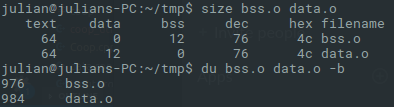
\includegraphics[width=0.5\textwidth, height=0.2\textwidth]{PICs/bss_data_comparison}
	\caption{Comparison of .bss and .data sizes for different initializations.}
	\label{seg_sizes}
\end{figure}
\linebreak
So for a splitted record \textit{Foo}, COOP will generate the following code injection in order to reserve the appropriate amount of contiguous memory space:
\begin{lstlisting}[language=C++,name={Code injection to generate contiguous block of memory for a record Foo's instances.},morekeywords={constexpr, size_t, coop_free_list},label={cont_mem_foo}]
constexpr size_t hot_size_plus_ali_NPC =
	coop::size_plus_alignments(N, alignment, element_size);

constexpr size_t cold_size_plus_ali_NPC =
	coop::size_plus_alignments(M, alignment, element_size);

char byte_data_Foo[hot_size_plus_ali_Foo + cold_size_plus_ali_Foo];

coop_free_list hot_free_list_instance_Foo(
	byte_data_Foo,
	byte_data_Foo+hot_size_plus_ali_Foo,
	alignment, sizeof(Foo));

coop_free_list cold_free_list_instance_Foo(
	byte_data_Foo+hot_size_plus_ali_Foo,
	byte_data_Foo+hot_size_plus_ali_Foo+cold_size_plus_ali_Foo,
	alignment, sizeof(coop_cold_fields_Foo));
\end{lstlisting}
Line 1 to 5 in \refcode{cont_mem_foo} determine how much memory in Byte we need to encompass all instances. In line seven we reserve the actual memory (uninitialized \textit{.bss}) which will be the combined sizes of the hot and the cold data for the record Foo. In line 9 to 17 we create the free list instances. \refcode{cont_mem_foo} also shows that we rely on some additional variables and computations here. The sizes of the memory block, that our free lists will manage, need to be adjusted to the way the free list will operate. As mentioned before in \refsec{field_weight_heuristics} to maximize access efficiency we will align our data. On the one hand we will pack as much instances together in a cache-line, on the other hand we will align those instance groups to the cache-lines alignment. This way we will possibly generate some padding between those instance groups, but we also guarantee, that the minimum amount of cache-lines is needed to load an instance. Disadvantageous strides will not lead to instances being separated among more cache-lines than necessary.\\
But now whenever this results in additional bytes for padding, we also effectively increased the necessary memory space to encompass all our entities. This is what the \textit{size\_plus\_alignments(size\_t number\_elements, size\_t alignment, size\_t element\_size)} function does. It takes the number of entities \textit{N} we expect during runtime (line 2), the \textit{alignment} that we will need to adjust on, and the \textit{element\_size} which will for example be the size of our record Foo.\\
The padding per instance group is dependent on whether or not the record's size is equal to, greater than or smaller than the cache-line size and defined like this (where \textit{S} is the record's size in Byte and \textit{CLS} the cache-line size):
\begin{align}
pad\_per\_group = \begin{cases}
	 0\text{ for } S == CLS\\
	(\myfloor{\frac{S}{CLS}} +1)\cdot CLS - S \text{ for } S > CLS\\
	CLS - (\myfloor{\frac{CLS}{S}}\cdot S) \text{ for } S < CLS
\end{cases}
\end{align} \\\\
The element size is also not just \textit{sizeof(Foo)}, because we need to consider the possibility for a very small record to be split. For example if record Foo consisted of only an int (4 Byte) and a long int (8 Byte) and we wanted to split the long int away, leaving us with a single 4 Byte. As we will see when we explore the free list, it depends on its entities to be at least the size of a pointer, so it can properly resemble a linked list. That's why the \textit{element\_size} will be the maximum of the size in Byte of Foo and a Foo pointer type, to guarantee the free list to work as intended.\\
When we have the padding per instance group we can calculate how much capacity we need to encompass all our elements including their groups' padding respectively (where \textit{m} is the number of instances per group, \textit{n} is the total amount of instances):
\begin{align}
	capacity = (m\cdot S + pad\_per\_group)\cdot \myceil{\frac{n}{m}}+CLS
\end{align}
The alignment is the target cache's alignment, which COOP will retrieve from the system on program start. On Unix systems information on the caches can be found in \textit{sys/devices/system/cpu/cpu}<CPU ID>\textit{/cache/index}<cache ID>. For example the file \textit{sys/devices/.../type} contains whether or not this cache is a data cache or not. The file \textit{coherency\_line\_size} will contain the cache-line size in Byte.\\
The same is done for the record Foo's new cold field struct. But the number of elements ratio between the record and its cold struct pendant will (shuold) not be 1:1 for reasons we will discuss in (TODO REF SEC emulating deep copies). For now its left to say, that \textit{N} and \textit{M} will be determined by the user, as we can not predict how many instances will actually be made.\\\\
Finally the free list instances are created (\refcode{cont_mem_foo} line 9 to 14) which will be given the byte range they will administer, as well as the target cache's line size and the 'chunk' size (which is just our record's size).
\begin{lstlisting}[language=C++,name={Shortened excerpt of COOP's freelist without asserts and some initialization code.},morekeywords={constexpr, size_t},label={free_list}]
	class coop_free_list	{
	...
	coop_fre_list(char *data_start, char *data_end, size_t alignment, size_t block_size){
		...
		for(size_t Ts = 0; free_ptr < end; free_ptr = *next)
		{
			if(++Ts > Ts_per_chunk)
			Ts = 1;
			
			*next =
				free_ptr+block_size+(Ts == Ts_per_chunk ? padding_to_next : 0);
			
			if(*next >= end){*next = nullptr; break;}
		}
		free_ptr = begin;
	}
	
	template<typename T> T * get()
	{
		T *ret = union_cast<T*>(free_ptr);
		free_ptr = *next;
		return ret;
	}
	
	void free(void *p)
	{
		char *tmp_ptr = free_ptr;
		free_ptr = union_cast<char*>(p);
		*next = tmp_ptr;
	}
private:
	union {
		char *free_ptr;
		char **next;
	};
	char * begin = nullptr;
	char * end = nullptr;
	};
\end{lstlisting}
The \textit{coop\_free\_list} itself will only have three fields. Two char pointers (\textit{begin} and \textit{end}) which will mainly be used for bounds checking and a union containing a char pointer \textit{free\_ptr} that can also be used as a pointer to a char pointer.\\
In their essence free lists are only linked lists. Linked lists usually contain several nodes, that are linked to their successors, sometimes their predecessors and depending on specific implementations even more pointers to relevant nodes like the list head and end. I classic introductions to linked lists, nodes are allocated dynamically and a linked list can therefore grow (and spread) over the free memory. A linked list's nodes usually contain a data element, that in our case would hold the concrete instance and one or more pointers to other nodes,so the list can be iterated by following the trail the pointers constitute. In the case of a free list we want to work with contiguous memory blocks instead. Also to further work towards beneficial cache behavior it utilizes the data's memory space to also contain the pointer information to other 'nodes'. Each respective memory range, that will encompass an instance, will actually contain the pointer to the next element, whenever it does not at the moment represent an existing instance \reffigp{free_list_in_memory}.\\
Since we especially want to handle single instance allocations and pack those into cache-line groups we will need further effort to ensure, that those groups are aligned optimally. \refcode{free_list}'s lines 3 to 15 contain an important part of the free lists constructor. Here we initially iterate over our entire range to set up the adjacency relations of our 'nodes'. Until this point we already determined the number of instances per cache-line group (or chunk). The free list instance will work with any data type, but will almost entirely work with char pointers to avoid unnecessary much templated code. However since 'generic' data types are often represented as \textit{T}, the number of instances per chunk will here be \textit{Ts\_per\_chunk}.\\
Starting at an address, that will initially be aligned to a cache-line we will treat it as a pointer to a char pointer instead of a char pointer, so we can emplace the information of where to find the next node in it (line 7 to 13). This is a simple operation, because we know the size of an instance (our \textit{block\_size}). Since the block size encodes Byte units we can just add it to the address of this iteration to get the address of the upcoming element. Doing so we will count towards the \textit{Ts\_per\_chunk}. When we exceed the number of elements in a cache-line group, instead of only adding the block\_size to the current address we will also add the necessary padding we determined earlier to jump towards the next aligned adress and start a new cache-line group \reffigp{free_list_in_memory}.\\
Treating the current address as a pointer to a char pointer is possible by accessing it through the union's \textit{char **next}. 
\begin{figure}[!htbp]
	\centering
	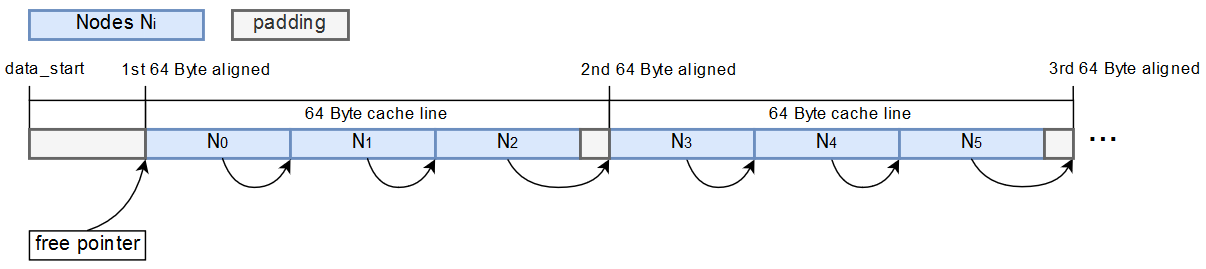
\includegraphics[width=0.86\textwidth, height=0.3\textwidth]{PICs/free_list_in_memory}
	\caption{The free list's layout in memory. Starting with a (possible) initial padding, the instances here represented by nodes will be grouped in a way, that a maximum amount of nodes fits a cache-line. Each group is again aligned to the cache-lines (here 64 Byte) to guarantee minimal loads.}
	\label{free_list_in_memory}
\end{figure}
To obtain a pointer to an element the free list provides the \textit{get} method which will simply return the actual free pointer and declare the 'next' node to be the currently free element (\refcode{free_list} line 18 to 23). It is equally easy to declare an instance's node as free space again, by caching the current free pointer in a temporary variable, setting the actual free pointer to the newly free address and declaring it's 'next' element as the cached variable (\refcode{free_list} line 25 to 30).

\subsubsection{Problematic fragmentation}
Just like the free memory ultimately our free list is prone to fragmentation, as soon, as the target program's instances 'die' more frequently as well as randomly. On the one hand we do not have to worry about a for loop trying to iterate over all the elements in the free list, by merely iterating an index variable over the original array, because our free list is injected into the code and therefore the target code will have no interaction with our free list other than the ones we intend to. But fragmentation still hurts us, as it will deteriorate the number of instances to cache-lines ratio. For example when we have three instances in a cache-line group and 'destroy' every first and second element our instance : cache-line ratio will effectively have gone from 3:1 to 1:1.\\\\
However as new elements are created the 'holes' in between the actual data blocks will refill. Pool allocators are inherently robust when it comes to fragmentation. So In certain situations, where our target program requires a bunch of instances, deletes a random subset of them regressing our instance : cache-line ratio to 1:1, we might encounter non optimal cache utilization.\\\\
This is a special case and might be neglected but a possible solution would be for our free list's to shift blocks of memory together. More specifically whenever an address is freed, we could take the last element and place it there. This way no matter how the \textit{get}/\textit{free} ratio of the target program would be, our data instances would be contiguous in memory. But its not that easy. Since we actually shifted the data a pointer to that data is now invalid.\\
To sustain the pointer it could either be a smart pointer, that observes the free list, reacting to changes, or our pool allocator could provide a second array solely consisting of pointers, to the original data array. The \textit{get} method would now return an index to the pointer array and the corresponding pointer would lead to the actual data. Whenever data is shifted the pointer array is traversed and updated accordingly. Whoever is holding an index to the pointer array, will now access the actual data through an additional indirection \mcp{gregory}{440}.\\
This could solve the fragmentation for special data lifetime patterns, but as mentioned above pool allocators are themselves quite robust to fragmentation so at this point its worth mentioning in case the pool allocator proves to be unqualified provide improved cache-utilization on its own.\\\\

Beneficial alignments of quasi continuous entity groups in memory can strongly affect a target programs cache utilization. With our heuristic considering the field's type sizes in Byte and the target cache's line-size we are moving away from making an educated guess towards calculating actual relations between a split and it's cache utilization. Measurements will show, that this approach is improving decision making on splits, however we will notice, that sometimes but not always our formulas are off a bit. Not meaning there is some sort of race condition going on. It rather depends on the project we are testing. To be more specific, it depends on the record declarations we are examining and the record sizes of the resulting split records. It might happen, that a target programs hot-record size is different from what we calculated when we tried to make a decision whether or not a split at a certain point is beneficial or not. How so?

\subsection{Structure Padding and field reordering}\label{structure_padding_and_field_reordering}
\begin{wrapfigure}[10]{r}{0.35\textwidth}
\vspace{-1cm}
\begin{lstlisting}[language=C++,numbers=none,name={Example field declarations to elaborate on structure padding},label={padding}]
char c;//+3B (possibly)
int i;

struct Foo{
	float f1;//+4B padding
	int *i_ptr;
	float f2;//+4B padding
};
\end{lstlisting}
\end{wrapfigure}
Whenever we work with fields of data, in C++ we do so by associating a type declaration to it. A field's type on first glance is nothing but a piece of information on how much actual space we need to reserve in memory to suffice our data's capacity. For \refcode{padding}'s char definition \textit{c} and int \textit{i} we could assume, that their layout in memory resembles their definitions in the source code, meaning there is one Byte for the char \textit{c} and the following next four Bytes are reserved for our int \textit{i}. Now sometimes and arguably most of the times this assumption will be valid, however depending on the particular address of \textit{c} in memory \textit{c}'s immediate succeeding Bytes will not belong to \textit{i}.\\\\
For our modern processors compilers lay out memory abiding alignment constraints in order to make accessing them faster \mc{padding}. We already talked about how COOP will align its data managed by the free list, so that an instance will be split upon a minimal amount of cache-lines. In the best case this means finding an instance's data on one cache-line entirely. This is done, so we can guarantee a minimal amount of main memory loads, when accessing our data. As we learned those main memory loads can be extremely expensive so aligning data in a way that reduces load operations can have a significant impact on run time performance.\\
This is also what compilers do, when generating machine code for our field declarations. Accordingly, any data type has a defined alignment requirement, that is the information on how to align this piece of memory to guarantee optimal access performance. While chars encompass only a single Byte, they can be placed anywhere without further alignment requirements. Four Byte floats, or ints for example must be placed at an address divisible by four; Eight Byte longs or doubles at addresses divisible by eight and so on. This is sometimes referred to as them being \textit{self-aligned}. One can manually arrange for the compiler to ignore alignment requirements (e.g. using pragma pack, or invoking the compiler with certain command line parameters), however this virtually always comes with punishment in terms of performance, so it is advised not to do so, unless its unavoidable \mc{padding}.\\
Not aligning a data type not only implicates unnecessary many loads, but also results in additional effort for the memory controller, since in order to operate on the data it must now mask, shift and logically OR the two together into a CPU register, so the imminent operations can treat it normally \mcp{gregory}{160}.\\\\
Lets come back to our example \refcode{padding}. In order to abide alignment requirements, depending on where char \textit{c} lays in memory, our char \textit{i} might follow a three Byte long hole of padding. The same goes for field declarations inside record definitions. While the float \textit{Foo::f1} is guaranteed to abide its alignment requirement (we will shortly see why) the int poitner \textit{Foo::i\_ptr} will need to follow a four Byte padding in order to be aligned correctly. Float \textit{f2} follows a higher alignment requirement, which suffices its own requirements (All alignment requirements are powers of two).\\
The compiler will add one last padding to this record definition, because it considers the possibility of struct \textit{Foo} to be used in continuous blocks of memory. In order not to invalidate the field paddings we need to ensure, that they are correct for each successional instance. This can be done by aligning the record to its highest field alignment requirement. For our struct \textit{Foo} this means, that in order to suffice the eight Byte alignment requirement we need trailing padding of an additional four Byte. Consequently the size of our struct \textit{Foo} is not 16, but 24 Byte. Defining \textit{Foo}'s fields in a different order could get rid of (in this case) unnecessary padding but essentially this explains how on certain test files COOP's methodology to determine a favorable split won't match the actual situation.\\
When considering a split for a certain subset of fields, there is not yet an actual compiled version of it. We do not have the means to call \textit{sizeof(non-existent-record)} on it, so either we implement a JIT compiler to momentarily compile a version of our record, or we consider structure padding our selfes. Merely summarizing the field's type sizes won't be enough, as it may disregard possible structure padding.\\
In \refsec{sig_groups} we defined our formula on how to determine whether or not a split at a certain point is favorable or not. In order for this formula to work properly it needs to consider a theoretical split-record's structure padding.\\
We have seen, that records can be defined in suboptimal ways. We have seen before in \refsec{rtasl} that padding just like unused data is effectively lost potential in terms of cache utilization and we also have the means to 'improve' the target definitions layout. COOP will in fact rearrange a record's field definitions in a descending order (descending alignment requirements) to avoid unnecessary structure padding. With this COOP is able to get rid of most padding Bytes.\\\\
In \refsec{bleh} (TODO REF SEC FUTURE WORK AND PROBLEMS) we will discuss some major problems that this approach implicates. Actually this topic really hints at why an optimization like this can \textbf{never} be considered 'legal' or safe in terms of C++ language compliance and we will see, why COOP will work fine in some situations but in principal can't work.






%\chapter{Quotes}
%\section{hennessy}
\subsection{principle of locality}
\textit{The	most important program property that we regularly exploit is the principle of
	locality: Programs tend to reuse data and instructions they have used recently. A
	widely held rule of thumb is that a program spends 90\% of its execution time in
	only 10\% of the code. An implication of locality is that we can predict with reasonable
	accuracy what instructions and data a program will use in the near future
	based on its accesses in the recent past. The principle of locality also applies to
	data accesses, though not as strongly as to code accesses.
	Two different types of locality have been observed. Temporal locality states
	that recently accessed items are likely to be accessed in the near future. Spatial
	locality says that items whose addresses are near one another tend to be referenced
	close together in time.}
\mcp{hennessy}{38}


%\section{drepper}
\subsection{cache layout}


\subsection{Lc Ld}
\textit{Even though most computers for the last several decades
	have used the von Neumann architecture, experience has
	shown that it is of advantage to separate the caches used
	for code and for data}
\mcp{Drepper}{14}
%\section{compilers}
\subsection{what is a compiler}
Simply stated, a compiler is a program that can read a program in one language - the source language - and translate it into an equivalent program in another language - the target language[...]. \mcp{aho}{1}

\subsection{evolution of programming languages}
\mcp{aho}{13}

\subsection{requirements to optimizations}
\mcp{aho}{16}

\subsection{optimizing compilers}
Programmers using a low-level language have more control over a computation and can, in principle, produce more efficient code. Unfortunately , lower-level programs are harder to write and - worse still - less portable, more prone to errors, and harder to maintain. Optimizing compilers include techniques to improve the performance of generated code, thus offsetting the inefficiency introduced by high-level abstractions. \mcp{aho}{17}

\subsection{compiler phases}


\subsection{compiler front end}
\begin{figure}[!htbp]
	\centering
	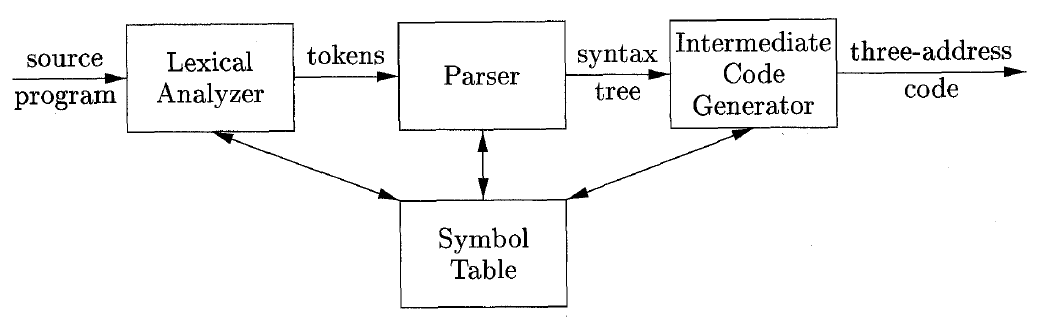
\includegraphics[width=1.0\linewidth]{PICs/compiler_front_end}
	\caption{Model of compiler front end \mcppic{aho}{41}.}\label{compiler_front_end}
\end{figure}

\subsection{AST}
In an \textit{abstract syntax tree} for an expression, each interior node represents an operator; the children of the node represent the operands of the operator. More generally, any programming construct can be handled by making up an operator for the construct and treating as operands the semantically meaningful components of that construct. \mcp{aho}{69}

\subsection{low level vs high level}
The more a language hides the hardware the less control it offers over it. Low-level languages interact more directly with the hardware (more control) thus enable one to write better performing code. But they are usually harder to write as well as less portable, more prone to errors, and harder to maintain \mcp{aho}{17}.\\


%
% Hier beginnen die Verzeichnisse.
%
\clearpage
\ifthenelse{\equal{\FHTWCitationType}{HARVARD}}{}{\bibliographystyle{gerabbrv}}
\bibliography{Literatur}
\clearpage

% Das Abbildungsverzeichnis
\listoffigures
\clearpage

% Das Tabellenverzeichnis
\listoftables
\clearpage

% Das Quellcodeverzeichnis
\listofcode
\clearpage

\phantomsection
\addcontentsline{toc}{chapter}{\listacroname}
\chapter*{\listacroname}
\begin{acronym}[XXXXX]
    \acro{ABC}[ABC]{Alphabet}
    \acro{WWW}[WWW]{world wide web}
    \acro{ROFL}[ROFL]{Rolling on floor laughing}
\end{acronym}

%
% Hier beginnt der Anhang.
%
\clearpage
\appendix
\chapter{Anhang A}
\clearpage
\chapter{Anhang B}
\end{document}